%%  LJMU LaTeX Thesis Template - Author: Martyn Bristow
%% Thesis.tex -- Main file - compile this with LaTeX
%% 

% Set up the document
\documentclass[a4paper, 11pt, oneside]{LJMU_Astro_Thesis}  % Use the "Thesis" style, based on the ECS Thesis style by Steve Gunn
\usepackage[english]{babel}
\usepackage[utf8x]{inputenc}
\usepackage[T1]{fontenc}

\usepackage{graphicx}
%\usepackage{braket}
\usepackage[english]{babel}
\usepackage{upgreek}
\usepackage{graphicx}
\usepackage{float}
\usepackage{natbib}
\usepackage{amsmath}
\usepackage{amssymb}
\usepackage{tabularx,ragged2e,booktabs,caption}
\usepackage{graphicx} % for images
\usepackage[font=small]{caption}
\usepackage{setspace}
\usepackage{epstopdf}
\usepackage{subcaption}

\graphicspath{{Figures/}}  % Location of the graphics files (set up for graphics to be in PDF format)

% Include any extra LaTeX packages required
\usepackage[square, numbers, comma, sort&compress]{natbib}  % Use the "Natbib" style for the references in the Bibliography
\usepackage{verbatim}  % Needed for the "comment" environment to make LaTeX comments
\usepackage{vector}  % Allows "\bvec{}" and "\buvec{}" for "blackboard" style bold vectors in maths
\hypersetup{urlcolor=black, colorlinks=true}  % Colours hyperlinks in blue, but this can be distracting if there are many links.
% Valid latex color: white, black, red, green, blue, cyan, magenta, yellow.

%% Custom definitions
\def\aap{Astronomy \& Astrophysics}
\def\apj{The Astrophysical Journal}
\def\mnras{Monthly Notices of the Royal Astronomical Society}
%% ----------------------------------------------------------------
\begin{document}
\frontmatter      % Begin Roman style (i, ii, iii, iv...) page numbering

% Set up the Title Page
\title  {Thesis Title}
\authors  {\texorpdfstring
            {\href{http://martynbristow.co.uk/}{Martyn Bristow}}
            {Martyn Bristow}
            }
\addresses  {\groupname\\\deptname\\\univname}  % Do not change this here, instead these must be set in the "Thesis.cls" file, please look through it instead
\date       {\today}
\subject    {}
\keywords   {}

\maketitle
%% ----------------------------------------------------------------

\setstretch{1.5}  % It is better to have smaller font and larger line spacing than the other way round

% Define the page headers using the FancyHdr package and set up for one-sided printing
\fancyhead{}  % Clears all page headers and footers
\rhead{\thepage}  % Sets the right side header to show the page number
\lhead{}  % Clears the left side page header

\pagestyle{fancy}  % Finally, use the "fancy" page style to implement the FancyHdr headers

\pagestyle{plain}
\pagenumbering{roman}
\setcounter{page}{2}
\include{preface}
\newpage
\input{declaration}
\newpage
\input{abstract}
\newpage
%\input{publications}
%\newpage
\input{acknowledgements}
\newpage
%% ----------------------------------------------------------------
% Declaration Page required for the Thesis, your institution may give you a different text to place here
\Declaration{

\addtocontents{toc}{\vspace{1em}}  % Add a gap in the Contents, for aesthetics

I, AUTHOR NAME, declare that this thesis titled, `THESIS TITLE' and the work presented in it are my own. I confirm that:

\begin{itemize} 
\item[\tiny{$\blacksquare$}] This work was done wholly or mainly while in candidature for a research degree at this University.
 
\item[\tiny{$\blacksquare$}] Where any part of this thesis has previously been submitted for a degree or any other qualification at this University or any other institution, this has been clearly stated.
 
\item[\tiny{$\blacksquare$}] Where I have consulted the published work of others, this is always clearly attributed.
 
\item[\tiny{$\blacksquare$}] Where I have quoted from the work of others, the source is always given. With the exception of such quotations, this thesis is entirely my own work.
 
\item[\tiny{$\blacksquare$}] I have acknowledged all main sources of help.
 
\item[\tiny{$\blacksquare$}] Where the thesis is based on work done by myself jointly with others, I have made clear exactly what was done by others and what I have contributed myself.
\\
\end{itemize}
 
 
Signed:\\
\rule[1em]{25em}{0.5pt}  % This prints a line for the signature
 
Date:\\
\rule[1em]{25em}{0.5pt}  % This prints a line to write the date
}
\clearpage  % Declaration ended, now start a new page

%% ----------------------------------------------------------------
% The "Funny Quote Page"
\pagestyle{empty}  % No headers or footers for the following pages

\null\vfill
% Now comes the "Funny Quote", written in italics
\textit{``Write a funny quote here.''}

\begin{flushright}
If the quote is taken from someone, their name goes here
\end{flushright}

\vfill\vfill\vfill\vfill\vfill\vfill\null
\clearpage  % Funny Quote page ended, start a new page
%% ----------------------------------------------------------------

% The Abstract Page
\addtotoc{Abstract}  % Add the "Abstract" page entry to the Contents
\abstract{
\addtocontents{toc}{\vspace{1em}}  % Add a gap in the Contents, for aesthetics

The Thesis Abstract is written here (and usually kept to just this page). The page is kept centered vertically so can expand into the blank space above the title too\ldots

}
\chapter{Units and terminology}
Unless stated otherwise, all quantities will be described in CGS units (masses in grams, lengths in centimetres, times in seconds, energies in ergs).
$M$ : mass
$M_{odot} = 1.989 \times 10^{33} \textnormal{g}$ : solar mass
$L$ : luminosity
$L_{odot} = 3.842 \times 10^{33} \textnormal{erg s^{-1}}$ : solar luminosity
$g$ : gravity
$R$ : radius
$G = 6.6723 \times 10^{-8} \textnormal{cm^{3}g^{-1}s^{-2}}$ : gravitational constant
$\sigma_{SB} = 5.678 \times 10^{-5} \textnormal{erg cm^{-2}K^{-4}s^{-1}}$ : Stefan-Boltzmann constant

\chapter{Introduction}
\section{Motivation}
As the light emitted from a star travels towards a distant observer, its intensity, or flux, $F$ decreases with distance $d$ via an inverse-square law:

\begin{equation}
\label{flux_def}
F = \frac{L}{4 \pi d^{2}}
\end{equation}

where $L$ is the star's luminosity, which is an intrinsic property of the star (i.e., independent of the observer).
However, the interstellar medium is composed of many different structures, such as diffuse gas clouds, that can absorb or scatter light passing through, depending on the wavelength of the light.

\section{Background}
No telescope can view the sky at all spectral wavelengths - it would be wholly impractical due to the sheer number of sources across the spectrum, as well as the fact that telescope resolution depends on the wavelength of the incoming light. Therefore, modern telescopes are equipped with a system of filters or bands, which allow only light within a narrow range of wavelengths. In a filter system, the individual filters are designed to operate best at different wavelengths. The system will be therefore have the following properties:
\begin{itemize}
\item the filters cover a much wider range of spectral wavelengths when combined than a single filter would alone; this is used to observe sources at different wavelengths to determine its colour ** (see Section ***).
\item 
\end{itemize}
Filters - Johnson, ACS, WFC/UVIS, Gaia
Filter response functions.

\section{Previous studies}
**Cardelli et al. (1989) produced empirical equations to accurately describe the ratio of extinction coefficients in a chosen filter $X$ ($A_{X}$) and the Johnson-$V$ filter ($A_{V}$), respectively.



\chapter{Theory}
\section{Extinction definition}
Extinction is defined using the standard astronomical system of flux magnitudes. In general, the difference between two flux measurements, $F_{1}$ and $F_{2}$, in magnitudes, is expressed as:
\begin{equation}
\label{mags_def}
m_{1} - m_{2} = -2.5\log \left( \frac{F_{1}}{F_{2}} \right)
\end{equation}

where $m_{1}$ and $m_{2}$ are the magnitudes for $F_{1}$ and $F_{2}$, respectively. However, the flux of a source varies naturally with the distance to the observer (see Equation \ref{flux_def}). To account for this, the distances to the nearest stars was determined independently of their flux, by their parallax from Earth. This gives each astronomical object two characteristic flux measurements. These are the apparent magnitude, $m$, and the absolute magnitude, $M$. The apparent magnitude is the flux magnitude of a source, as observed by the telescope. The absolute magnitude is the projected flux magnitude of the same source if it were to be placed at a distance of 10 parsecs (pc) from the telescope, thus accounting for the distances The relation between these quantities if there is zero extinction can be found by combining Equations \ref{flux_def} and \ref{mags_def}:
% In general, the extinction coefficient $A$ is defined relative to two ubiquitous astrophysical quantities.
\begin{equation}
\label{distance_modulus}
m - M = -2.5\log \left( (\frac{10\textnormal{pc}}{d})^{2} \right) = 5log( (d/\textnormal{pc}) - 5
\end{equation}

The quantity ($m - M$) is known as the distance modulus. It is particularly useful for observing stellar populations, as stars within a single-age population are easily classified using their position on the theoretical Hertzsprung-Russell (HR) diagram or ***some of its observational equivalents, known as colour-magnitude diagrams (CMDs). In the HR diagram, stars of a given age and metallicity are plotted in the luminosity-effective temperature ($L-T_{\textnormal{eff}}$) plane. An example of a HR diagram is shown in Figure ****. It can be seen that all stars lie on a single, complicated line, known as an isochrone. Isochrones for different population ages and metallicities are calculated using theoretical stellar models for the largest possible spread of initial stellar masses. An isochrone in the HR diagram has a number of distinct features:
\begin{itemize}
\item Most stars, including the coolest and least-luminous ones, follow a tight pattern of luminoaity increasing with temperature. This is known as the main sequence (MS)
\item This pattern stops as the luminosity continues to increase slowly but with decreasing temperature. The end of the MS is called the main-sequence turn-off (MSTO), which is followed by the sub-giant branch (SGB).
\item After the SGB, the gradient becomes much steeper, with temperate decreasing and luminosity rapidly increasing. This is the red-giant branch (RGB).
\item At the tip of the RGB, stars start becoming fainter and their temperatures increase. Eventually, their is a sequence of stars with near-constant luminosity but a range of effective temperatures. This is the horizontal branch (HB).
\item After the horizontal branch, there is again a rapid increase in luminosity accompanied by a slow decrease in temperature. This is the asymptotic giant branch (AGB).
\end{itemize}

It should be noted that the distance modulus in Equation \ref{distance_modulus} does not include extinction. To link the apparent magnitude to extinction, it is necessary to separate the distance modulus from the observed apparent magnitude, $m_{obs}$. This can be done by defining the intrinsic apparent magnitude, $m_{0}$, such that:

\begin{equation}
\label{intrinsic_app_mag}
m_{0} - M = 5\log( (d/\textnormal{pc}) - 5
\end{equation}

i.e., the distance modulus is solely dependent on the distance to the  sources. Therefore, the extinction $A$ can be defined as:

\begin{equation}
\label{intrinsic_app_mag}
A = m_{obs} - m_{0}
\end{equation}

This fits with the definition of interstellar extinction given earlier, i.e. as the flux lost solely due to scattering and absorption in the interstellar medium.

\section{Bolometric corrections}
All the equations in Section ****, including those for extinction, are not useful when applied to telescopes, as any filter will only detect a small fraction of the stellar flux across all wavelengths (known as the bolometric stellar flux) that reaches the telescope. The missing information resulting from this observational constraint renders it difficult to determine the interstellar extinction. These constraints much be mitigated before an accurate value of the extinction coefficient can be determined. Bolometric corrections are employed for this purpose.

The use of bolometric corrections requires the detailed knowledge of stellar spectra least susceptible to significant extinction, i.e., nearby stars with high apparent fluxes. Only with complete knowledge of the spectrum from a reference star can the true spectrum of a distant star with unknown extinction be calculated. The spectra of these stars can be computed by using a grid of predicted fluxes from a stellar atmosphere model, the grid being composed of the stellar parameters known to change emission in stellar atmospheres. These are effective temperature, surface gravity and metallicity. For all filter systems studied in this project, the nearby star Vega was used as the reference object.

The effective temperature ($T_{\textnormal{eff}}$) of a star is defined as the temperature of a black body which produces the closest matching bolometric spectrum to that of the star. This approximation is valid because all stars have been observed to have spectra that closely resemble those of black bodies, with the notable exception of atmospheric absorption lines.
\begin{equation}
L = 4 \pi R^{2} \sigma_{SB} T_{\textnormal{eff}}^{4}
\label{Teff_def}
\end{equation}
Effective temperature has an effect on interstellar extinction due to its strong effect on the stellar luminosity and, hence, the flux. For a higher flux, more photons are likely to interact with the ISM, hence a higher extinction coefficient.

The metallicity of a star is defined as the fractional abundance of heavy elements, often approximated by iron alone, relative to the star's hydrogen abundance, compared to that of the Sun. The abundances are determined by the strength of the elements' characteristic atomic absorption lines in the stellar spectra.

\begin{equation}
\textnormal{[Fe/H]} = \log(N_{Fe}/N_{H}) - \log(N_{Fe,\odot}/N_{H,\odot})
\label{FeH_def}
\end{equation}

Since the output is logarithmic, a value of [Fe/H] = 0 indicates solar metallicity. An increase in metallicity would cause the corresponding absorption lines to be stronger, thus reducing the observable flux.

The surface gravity ($g$) of a star is defined at the stellar surface:

\begin{equation}
g = frac{GM_{*}}{R_{*}^{2}}
\label{g_def}
\end{equation}

A higher surface gravity represents a surface with a higher atomic number density. This environment produces a shorter mean free path for photons overall, meaning a smaller collision timescale. If the timescale is sufficiently small, the limit provided by Heisenberg's Uncertainty Principle causes an increase in the uncertainty of the energy absorbed by the atomic electron during the interaction with the photon:

\begin{equation}
\DeltaE \Deltat \approx h/(4\pi)
\label{heisenberg}
\end{equation}

This effect, known as ``pressure broadening'', causes a symmetrical distribution of absorption energies (and wavelengths) about the normal emission energy for that particular atomic state. This means fewer photons pass through the surface, thereby reducing the surface flux.

After accounting for a general extinction effect on an object's emission, its apparent magnitude in a given filter $X$ (i.e. wavelength range, which we define as increasing from $\lambda _{1}$ to $\lambda _{2}$) is given by:

\begin{equation}
m_{X} = -2.5 \log_{10} \left(\frac{ \int_{\lambda_{1}}^{\lambda_{2}} f_{\lambda} \left( 10^{-0.4 A_{X,\lambda}} \right) S_{\lambda} d\lambda }{ \int_{\lambda_{1}}^{\lambda_{2}} f_{\lambda}^{0} S_{\lambda} d\lambda }\right) + m_{X}^{0}
\label{app_mag_def}
\end{equation}

where $f_{\lambda}$ represents the monochromatic flux at a given wavelength $\lambda$ at the observer distance, $A_{X,\lambda}$ is the extinction value as a function of wavelength, $S_{\lambda}$ is the response function and $f_{\lambda}^{0}$ and $m_{X}^{0}$ represent the monochromatic flux and apparent magnitude, respectively, of a known reference object in $X$.

%Since our goal, ultimately, is to document potential effects of fundamental stellar properties upon observables, we need to connect the observational and idealised scenarios, for which we use bolometric corrections.

To derive the equation linking a bolometric correction with the extinction parameter, we start with the definition of a bolometric correction in a filter $X$, which is denoted by $BC_{X}$:

\begin{equation}
BC_{X} \equiv M_{\textnormal{bol}} - M_{X}
\label{BC_def}
\end{equation}

where $M_{X}$ is the absolute magnitude of the object in $X$ and $M_{\textnormal{bol}}$ is its (predicted) absolute bolometric magnitude, defined relative to the Sun using:

\begin{equation}
M_{\textnormal{bol}} = M_{\textnormal{bol},\odot} - 2.5 \log_{10} \left( \frac{4\pi R^{2}F_{\textnormal{bol}}}{L_{\odot}} \right)
\label{mbol_sun}
\end{equation}

where  $F_{\textnormal{bol}}$ is the bolometric stellar flux at its surface, $R$ is the stellar radius, $M_{\textnormal{bol},\odot}$ is the solar absolute bolometric magnitude, which is assumed in this work to have a value of 4.75 and $L_{\odot}$ is the solar luminosity, for which a value of $3.844 \times 10^{33}$ erg s$^{-1}$ is used. Bolometric corrections can be expressed as a function of extinction using the universal definition of $M_{X}$ in terms of $m_{X}$ and the distance $d$ to the source:

\begin{equation}
M_{X} = m_{X} - 2.5 \log_{10}\left( \left( \frac{d}{10 \textnormal{pc}} \right)^{2} \right),
\label{abs_mag_def}
\end{equation}

together with the equation $f_{\lambda}d^{2}=F_{\lambda}R^{2}$, where $F_{\lambda}$ is the monochromatic flux at $\lambda$ at the stellar surface. This gives the final function for a bolometric correction for filter $X$:

\begin{align}
\begin{split}
BC_{X} &= M_{\textnormal{bol},\odot} - m_{X}^{0} - 2.5 \log_{10} \left( \frac{4\pi R^{2}F_{\textnormal{bol}}}{L_{\odot}} \right) \\
&+ 2.5 \log_{10} \left( \frac{\int_{\lambda_{1}}^{\lambda_{2}} F_{\lambda} \left( 10^{-0.4 A_{X,\lambda}} \right) S_{\lambda} d\lambda}{\int_{\lambda_{1}}^{\lambda_{2}} f_{\lambda}^{0} S_{\lambda} d\lambda} \right)
\label{BC_extinc}
\end{split}
\end{align}

For a filter $X$, the extinction parameter $A_{X} = A_{X,\lambda}$ must be calibrated relative to a known value. In this work we will input a value of the extinction in the well-studied Johnson-$V$ filter, $A_{V}$. To extract $A_{X}$, we use the simple relation:

\begin{equation}
A_{X} = \left( \frac{A_{X}}{A_{V}} \right) A_{V}
\label{ratio_eq}
\end{equation}

together with the chosen value of $A_{V}$ (for this project the values were $A_{V} =$ 0, 1 - note that $BC_{X}(A_{V}=0)$ effectively assumes no extinction), before taking the difference between the two $BC_{X}(A_{V})$, giving the following equation:

\begin{align}
\begin{split}
BC_{X}(0) - BC_{X}(A_{V}) &= 2.5 \log_{10} \left( \frac{\int_{\lambda_{1}}^{\lambda_{2}} F_{\lambda}  S_{\lambda} d\lambda}{\int_{\lambda_{1}}^{\lambda_{2}} F_{\lambda}\left( 10^{-0.4 \left(A_{X,\lambda}/A_{V}\right)A_{V}} \right) S_{\lambda} d\lambda} \right)
\\ &\approx \left(A_{X}/A_{V}\right)A_{V}
\label{BCs_diff}
\end{split}
\end{align}

****average over the wavelength interval $[\lambda_{1},\lambda_{2}]$ which is a valid assumption \citep{2008PASP..120..583G}, even for the wide-field Hubble filters being studied in this work.

\section{Methodology}
\subsection{Software used}
Python 2.7
FORTRAN 77 code
ATLAS9
BaSTI
\subsection{Finding & fitting functions}
Guesswork!
\subsection{Isochrone data fitting}
BaSTI models - transforming grid variables
DR2 Babusiaux data, errors

\begin{equation}
\label{Teff_def}
L = 
\end{equation}

\begin{equation}
\label{gravity_def}
g = 
\end{equation}
\section{Results and discussion}
\subsection{Extinction coefficient models}

\begin{table}
\begin{center}
\begin{tabular}{cccccc}
\hline
%\multirow{2}{*}{System} & \multirow{2}{*}{Filter} & \multirow{2}{*}{$A_{1}$ function} & \multicolumn{3}{c}{$A_{1}$ coefficients} \\ \cline{4-6}
%\textbf{Filter} \\
System & Filter & $A_{1}$ function & & $A_{1}$ coefficients & \\
 & & & $a$ & $b$ & $c$ \\
\hline

& F435W & pow & -(3.381$\pm$0.733)$\times 10^{4}$ & -1.394$\pm$0.026 & 1.040$\pm$0.001 \\
& F475W & pow & -457.6$\pm$64.9 & -0.9000$\pm$0.0172 & 1.247$\pm$0.002 \\
& F555W & pow & -(4.383$\pm$0.871)$\times 10^{3}$ & -1.361$\pm$0.023 & 0.6771$\pm$0.0002 \\
ACS & F606W & pow & -(4.383$\pm$0.871)$\times 10^{3}$ & -1.361$\pm$0.023 & 0.6771$\pm$0.0002 \\
& F625W & pow & -(3.381$\pm$0.733)$\times 10^{4}$ & -1.394$\pm$0.026 & 1.040$\pm$0.001 \\
& F775W & pow & -457.6$\pm$64.9 & -0.9000$\pm$0.0172 & 1.247$\pm$0.002 \\
& F814W & pow & -(4.383$\pm$0.871)$\times 10^{3}$ & -1.361$\pm$0.023 & 0.6771$\pm$0.0002 \\ \hline
% -2.32428259e+02  -1.07634845e-03   2.93338391e+00
% -1.28482746e+02  -1.03094181e-03   2.61038997e+00
% -9.72567775e-01  -3.51770388e-04   2.06004238e+00
% -5.33470924e+05  -1.66350652e+00   2.05158490e+00
% -1.51556105e+04  -1.58229494e+00   1.64765130e+00
% -0.59910717 -0.08070638  1.73786479
% -9.99999999e+04  -1.78304457e+00   1.35186267e+00
% -1.20707226e+05  -1.70657822e+00   1.22045256e+00
% -4.59655266e+05  -1.88059297e+00   1.07985380e+00
% -3.13655088e+05  -1.82928924e+00   9.64793923e-01
% -5.47562323e+05  -2.02950259e+00   8.78683006e-01
% -6.32767059e+03  -1.57627077e+00   6.56703339e-01
% -3.72711692e+03  -1.43145264e+00   6.15752594e-01
% -3.38142759e+04  -1.39444200e+00   1.03998507e+00
% -457.55192948   -0.89995256    1.24675509
% -4.38278161e+03  -1.36062232e+00   6.77129794e-01
& F218W & exp & -232.4$\pm$48.1 & -(1.076$\pm$0.043)$\times 10^{-3}$ & 2.933$\pm$0.007 \\
& F225W & exp & -128.5$\pm$13.8 & -(1.031$\pm$0.022)$\times 10^{-3}$ & 2.610$\pm$0.003 \\
& F275W & exp & 0.9726$\pm$0.0581 & -(3.518$\pm$0.109)$\times 10^{-4}$ & 2.060$\pm$0.001 \\
& F300X & pow & -(5.335$\pm$0.936)$\times 10^{5}$ & -1.664$\pm$0.021 & 2.052$\pm$0.001 \\
& F336W & pow & -(1.516$\pm$0.723)$\times 10^{4}$ & -1.582$\pm$0.056 & 1.648$\pm$0.001 \\
& F390W & pow & -0.5991$\pm$0.1494 & -0.08071$\pm$0.09090 & 1.738$\pm$0.309 \\
WFC3 & F438W & pow & -(1.000$\pm$0.463)$\times 10^{5}$ & -1.783$\pm$0.054 & 1.352$\pm$0.001 \\
& F475W & pow & -(1.207$\pm$0.379)$\times 10^{5}$ & -1.707$\pm$0.037 & 1.220$\pm$0.001 \\
& F555W & pow & -(4.560$\pm$1.490)$\times 10^{5}$ & -1.881$\pm$0.038 & 1.080$\pm$0.001 \\
& F606W & pow & -(3.137$\pm$0.911)$\times 10^{5}$ & -1.829$\pm$0.034 & 0.9648$\pm$0.0003 \\
& F625W & pow & -(5.476$\pm$3.709)$\times 10^{5}$ & -2.030$\pm$0.079 & 0.8787$\pm$0.0002 \\
& F775W & pow & -(6.328$\pm$4.571)$\times 10^{3}$ & -1.576$\pm$0.085 & 0.6567$\pm$0.0001 \\
& F814W & pow & -(3.727$\pm$1.381)$\times 10^{3}$ & -1.431$\pm$0.044 & 0.6158$\pm$0.0002 \\ \hline

& G & pow & -(3.381$\pm$0.733)$\times 10^{4}$ & -1.394$\pm$0.026 & 1.040$\pm$0.001 \\
Gaia & G\textsubscript{bp} & pow & -457.6$\pm$64.9 & -0.9000$\pm$0.0172 & 1.247$\pm$0.002 \\
& G\textsubscript{rp} & pow & -(4.383$\pm$0.871)$\times 10^{3}$ & -1.361$\pm$0.023 & 0.6771$\pm$0.0002 \\ \hline

\end{tabular}
\caption{Coefficient values produced by $A_{1}$ fitting}
\label{simpfunc_coeffs_table}
\end{center}
\end{table}

\subsection{Effect on isochrones}
\subsubsection{ACS} \label{ACS_isoc}

\begin{figure}[h]
\begin{center}
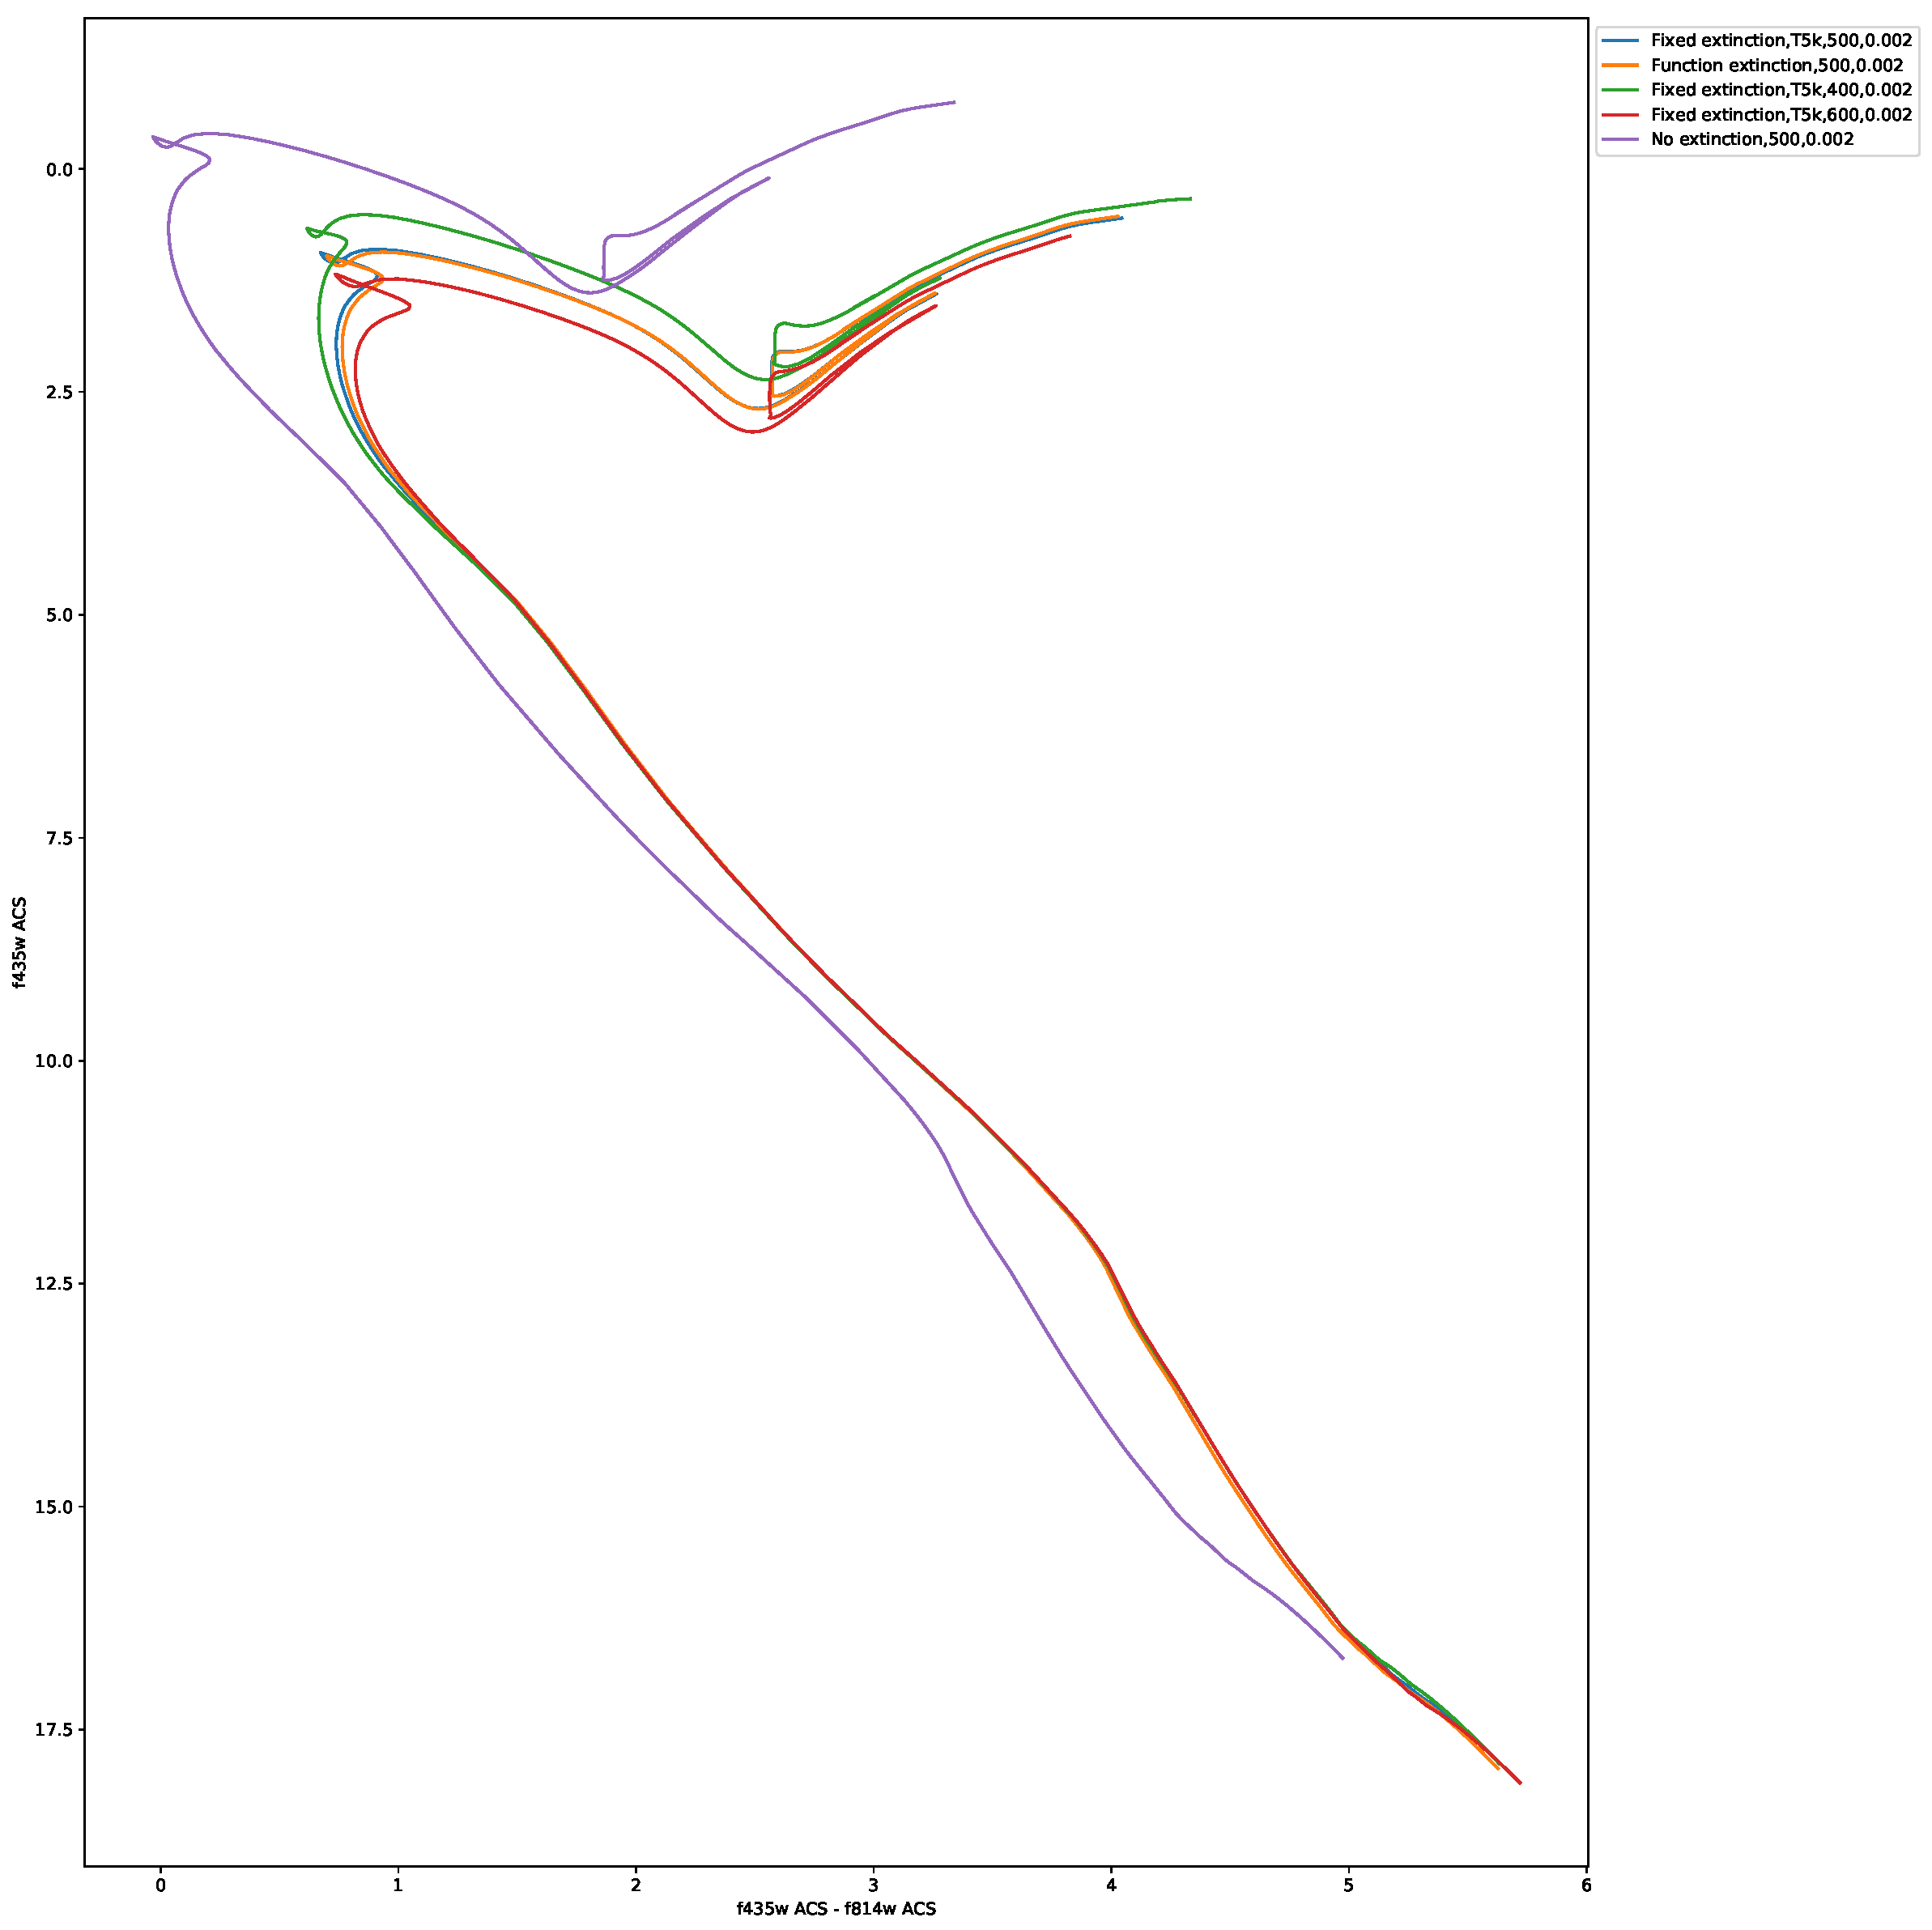
\includegraphics[scale=0.3]{../basti_isochrones_10_13Gyr/Extinction_T5k_FeH0fix_func_f435wACS_f435wACSmf814wACS_500_400_600_Myr_FeH_0p002_ref_noext_Av_1p0.pdf}
\caption{Ratios of $A_{X}/A{V}$ values for different $Z$ values compared with solar metallicity data at log($g$) = 5.0}
\label{acs_isoc_T5k}
\end{center}
\end{figure}

\begin{figure}[h]
\begin{center}
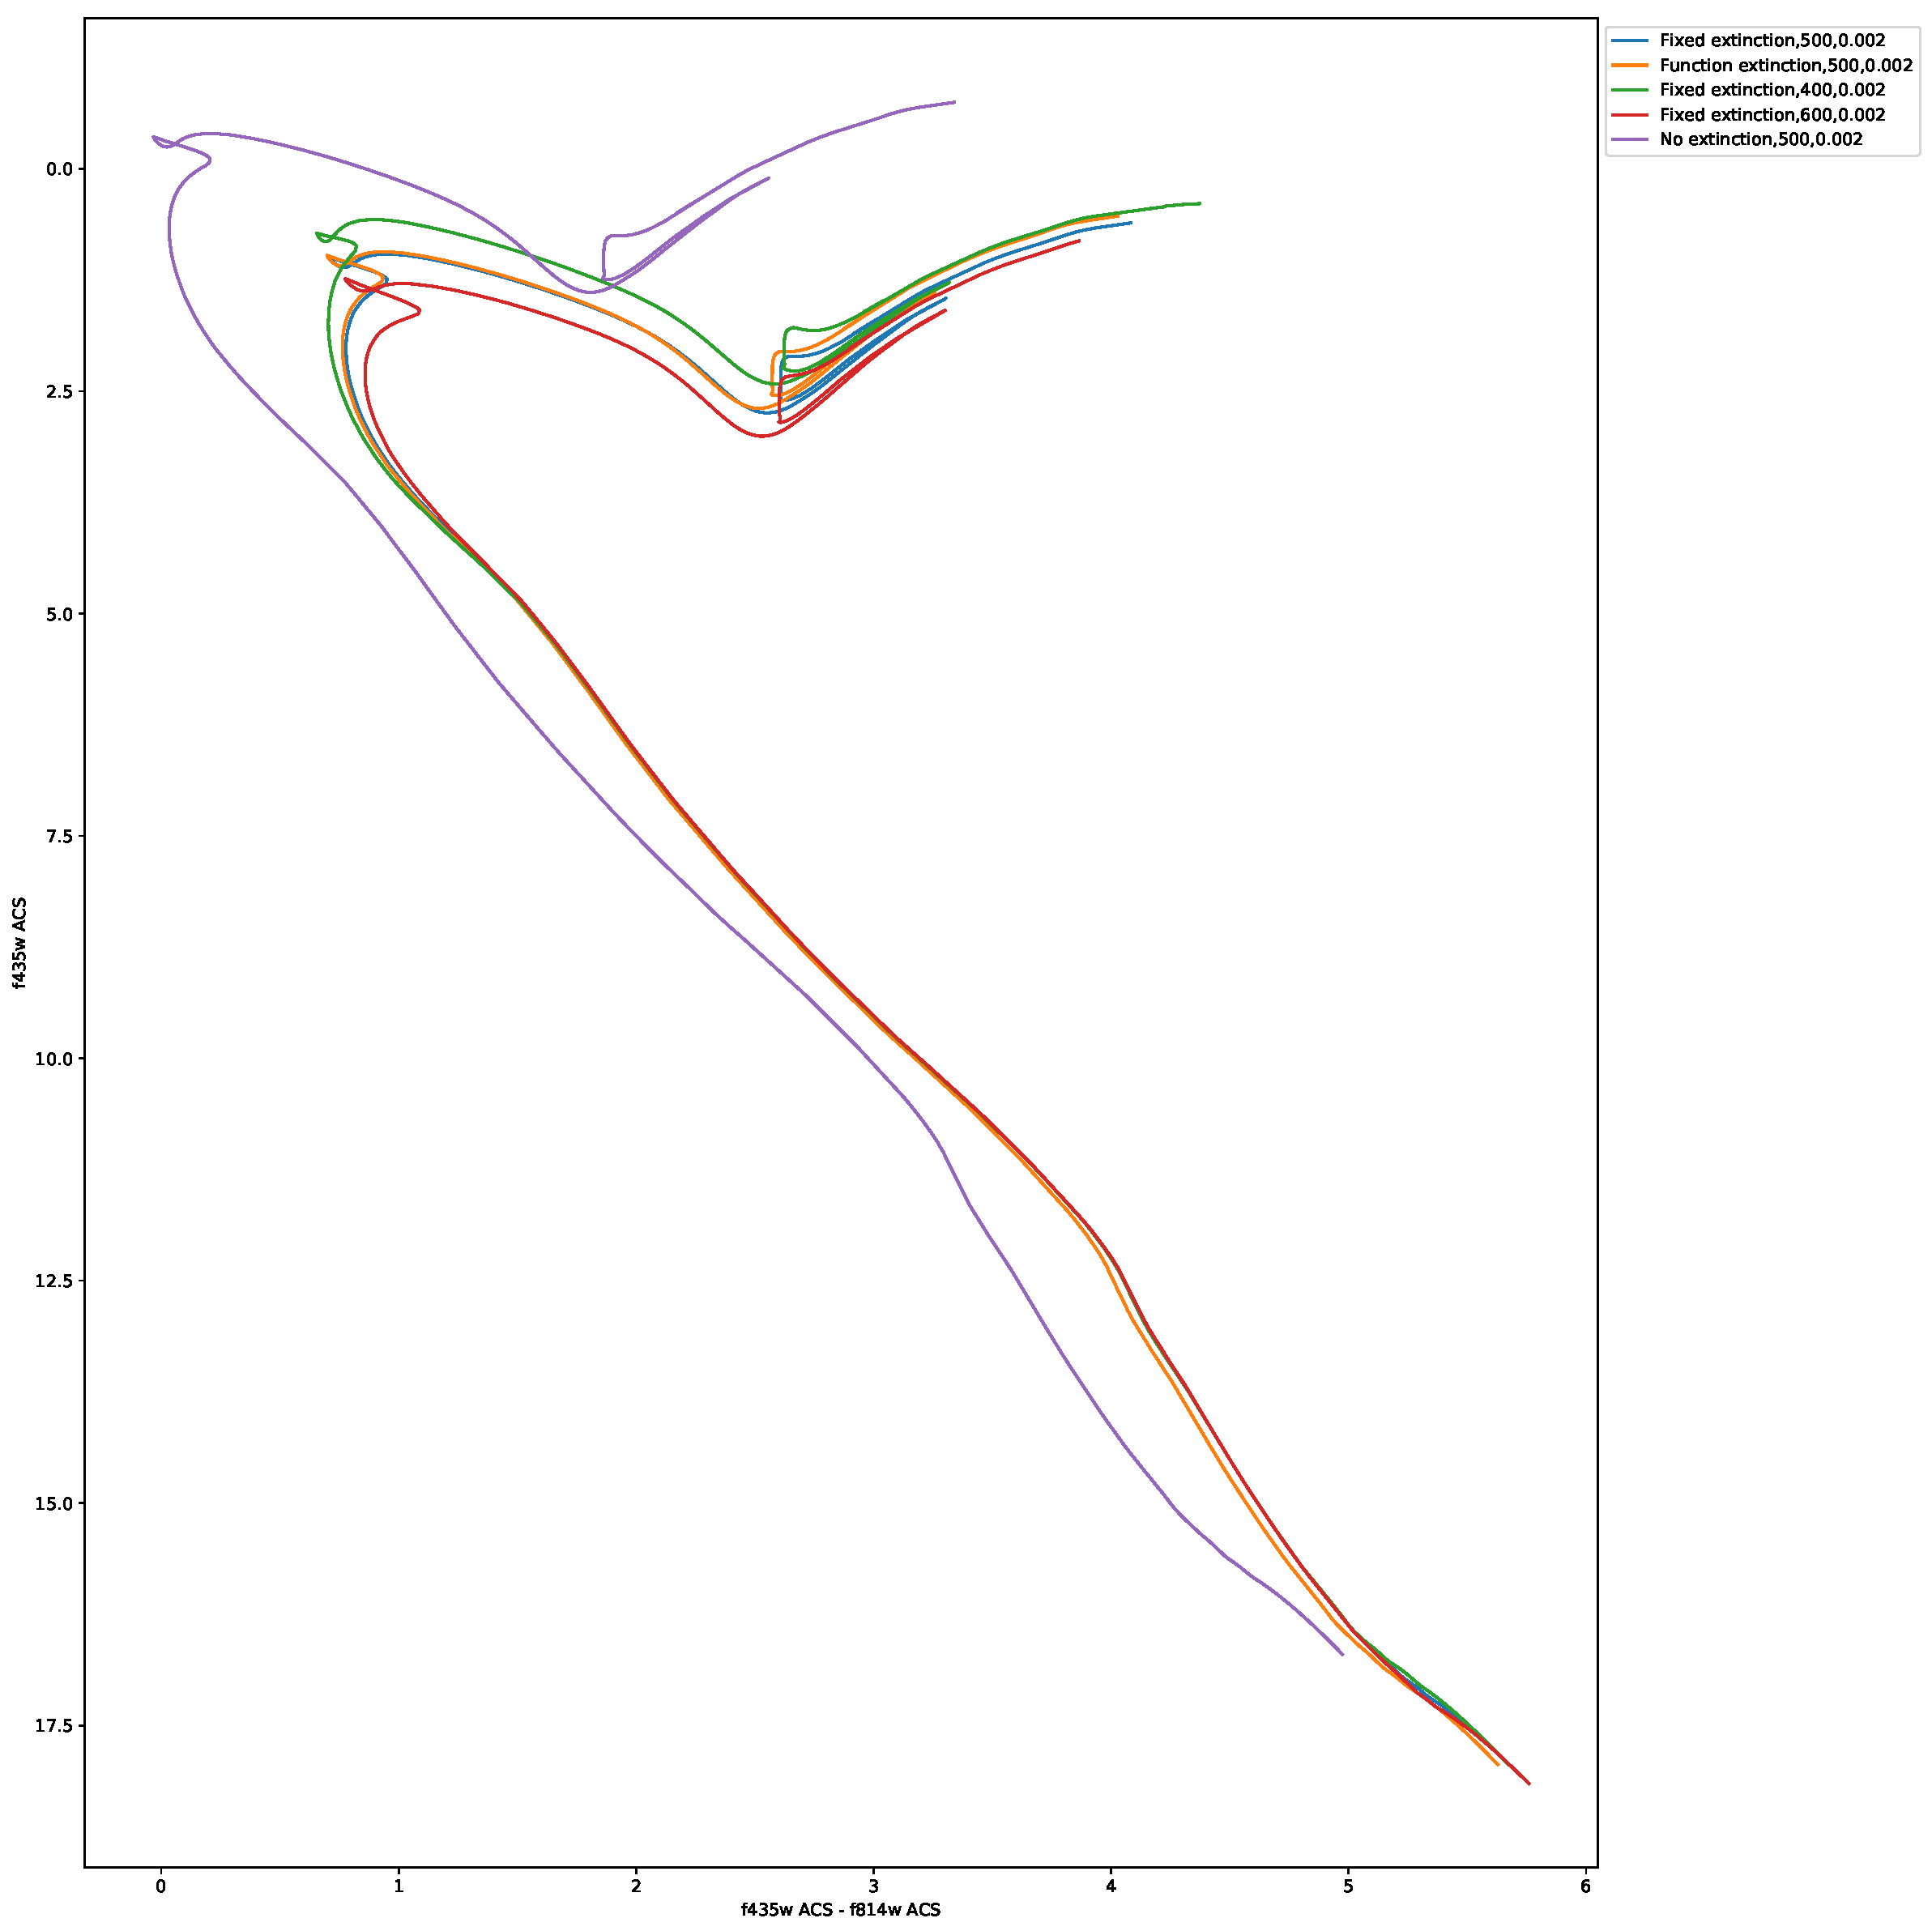
\includegraphics[scale=0.3]{../basti_isochrones_10_13Gyr/Extinction_T50k_FeH0fix_func_f435wACS_f435wACSmf814wACS_500_400_600_Myr_FeH_0p002_ref_noext_Av_1p0.pdf}
\caption{Ratios of $A_{X}/A{V}$ values for different $Z$ values compared with solar metallicity data at log($g$) = 5.0}
\label{acs_isoc_T50k}
\end{center}
\end{figure}

\subsubsection{WFC3} \label{WFC3_isoc}

\begin{figure}[h]
\begin{center}
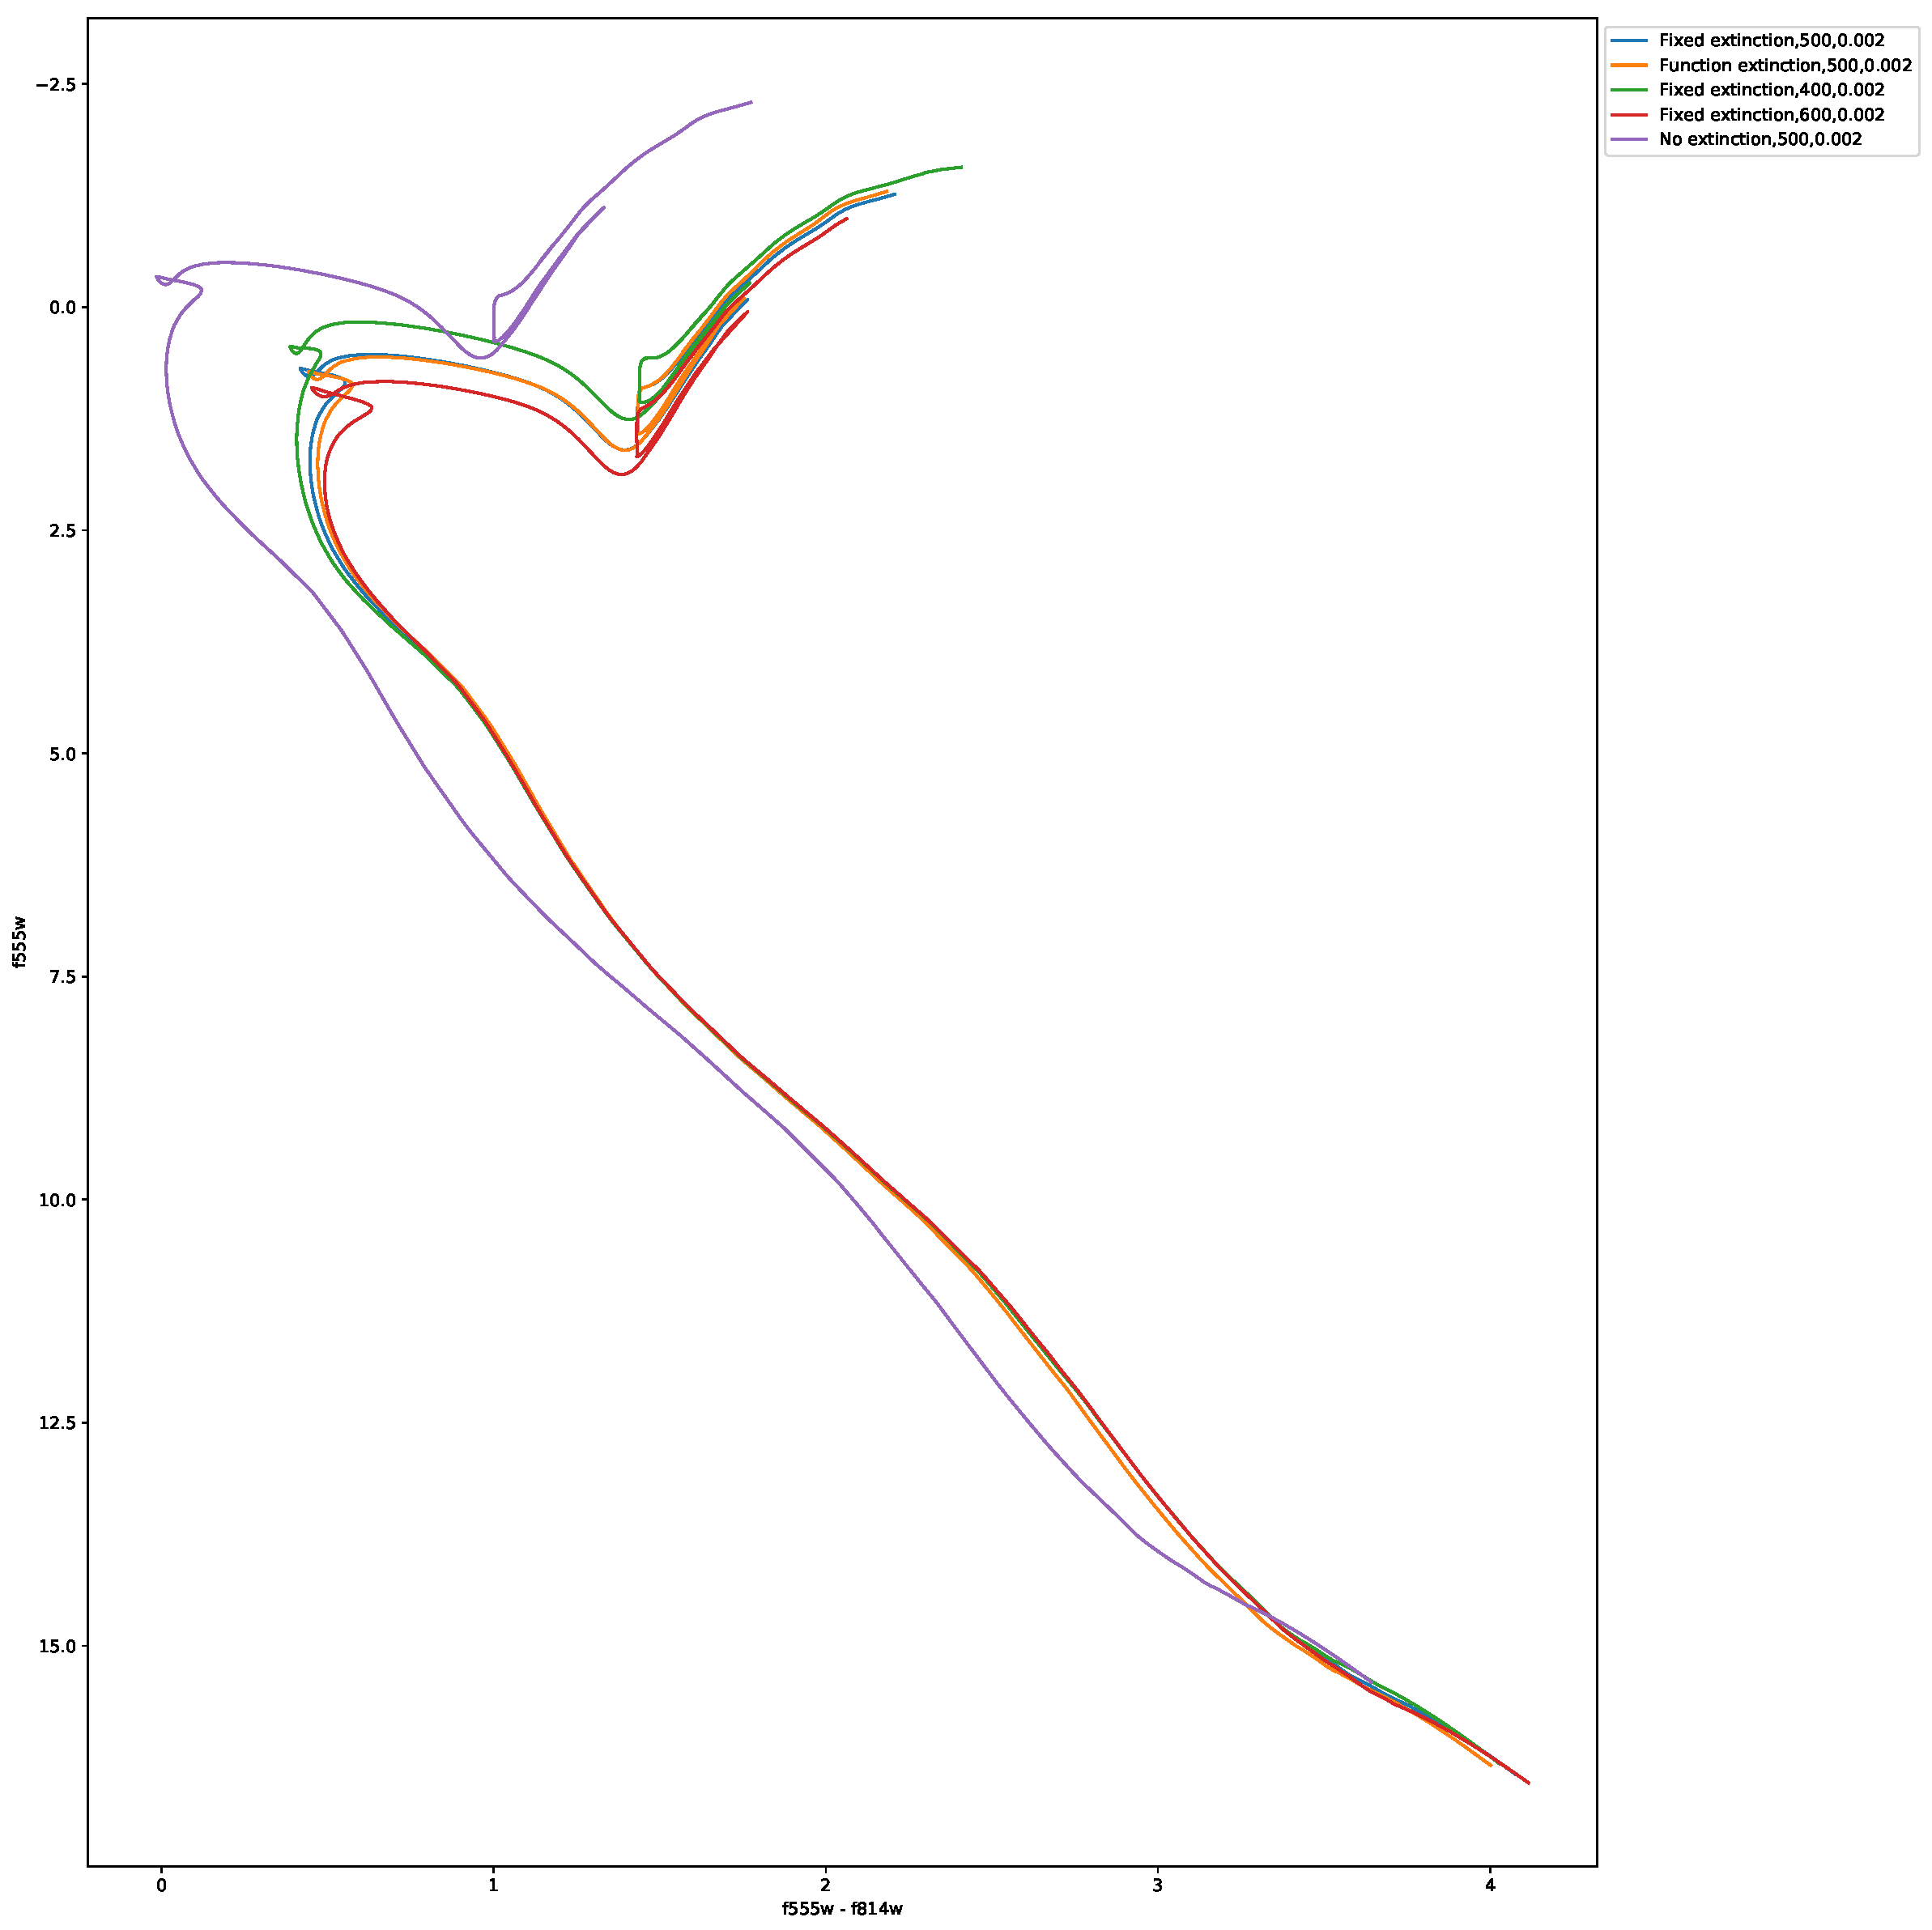
\includegraphics[scale=0.3]{../basti_isochrones_10_13Gyr/Extinction_T5k_FeH0fix_func_f555w_f555wmf814w_500_400_600_Myr_FeH_0p002_ref_noext_Av_1p0.pdf}
\caption{Ratios of $A_{X}/A{V}$ values for different $Z$ values compared with solar metallicity data at log($g$) = 5.0}
\label{wfc3_isoc1_T5k}
\end{center}
\end{figure}

\begin{figure}[h]
\begin{center}
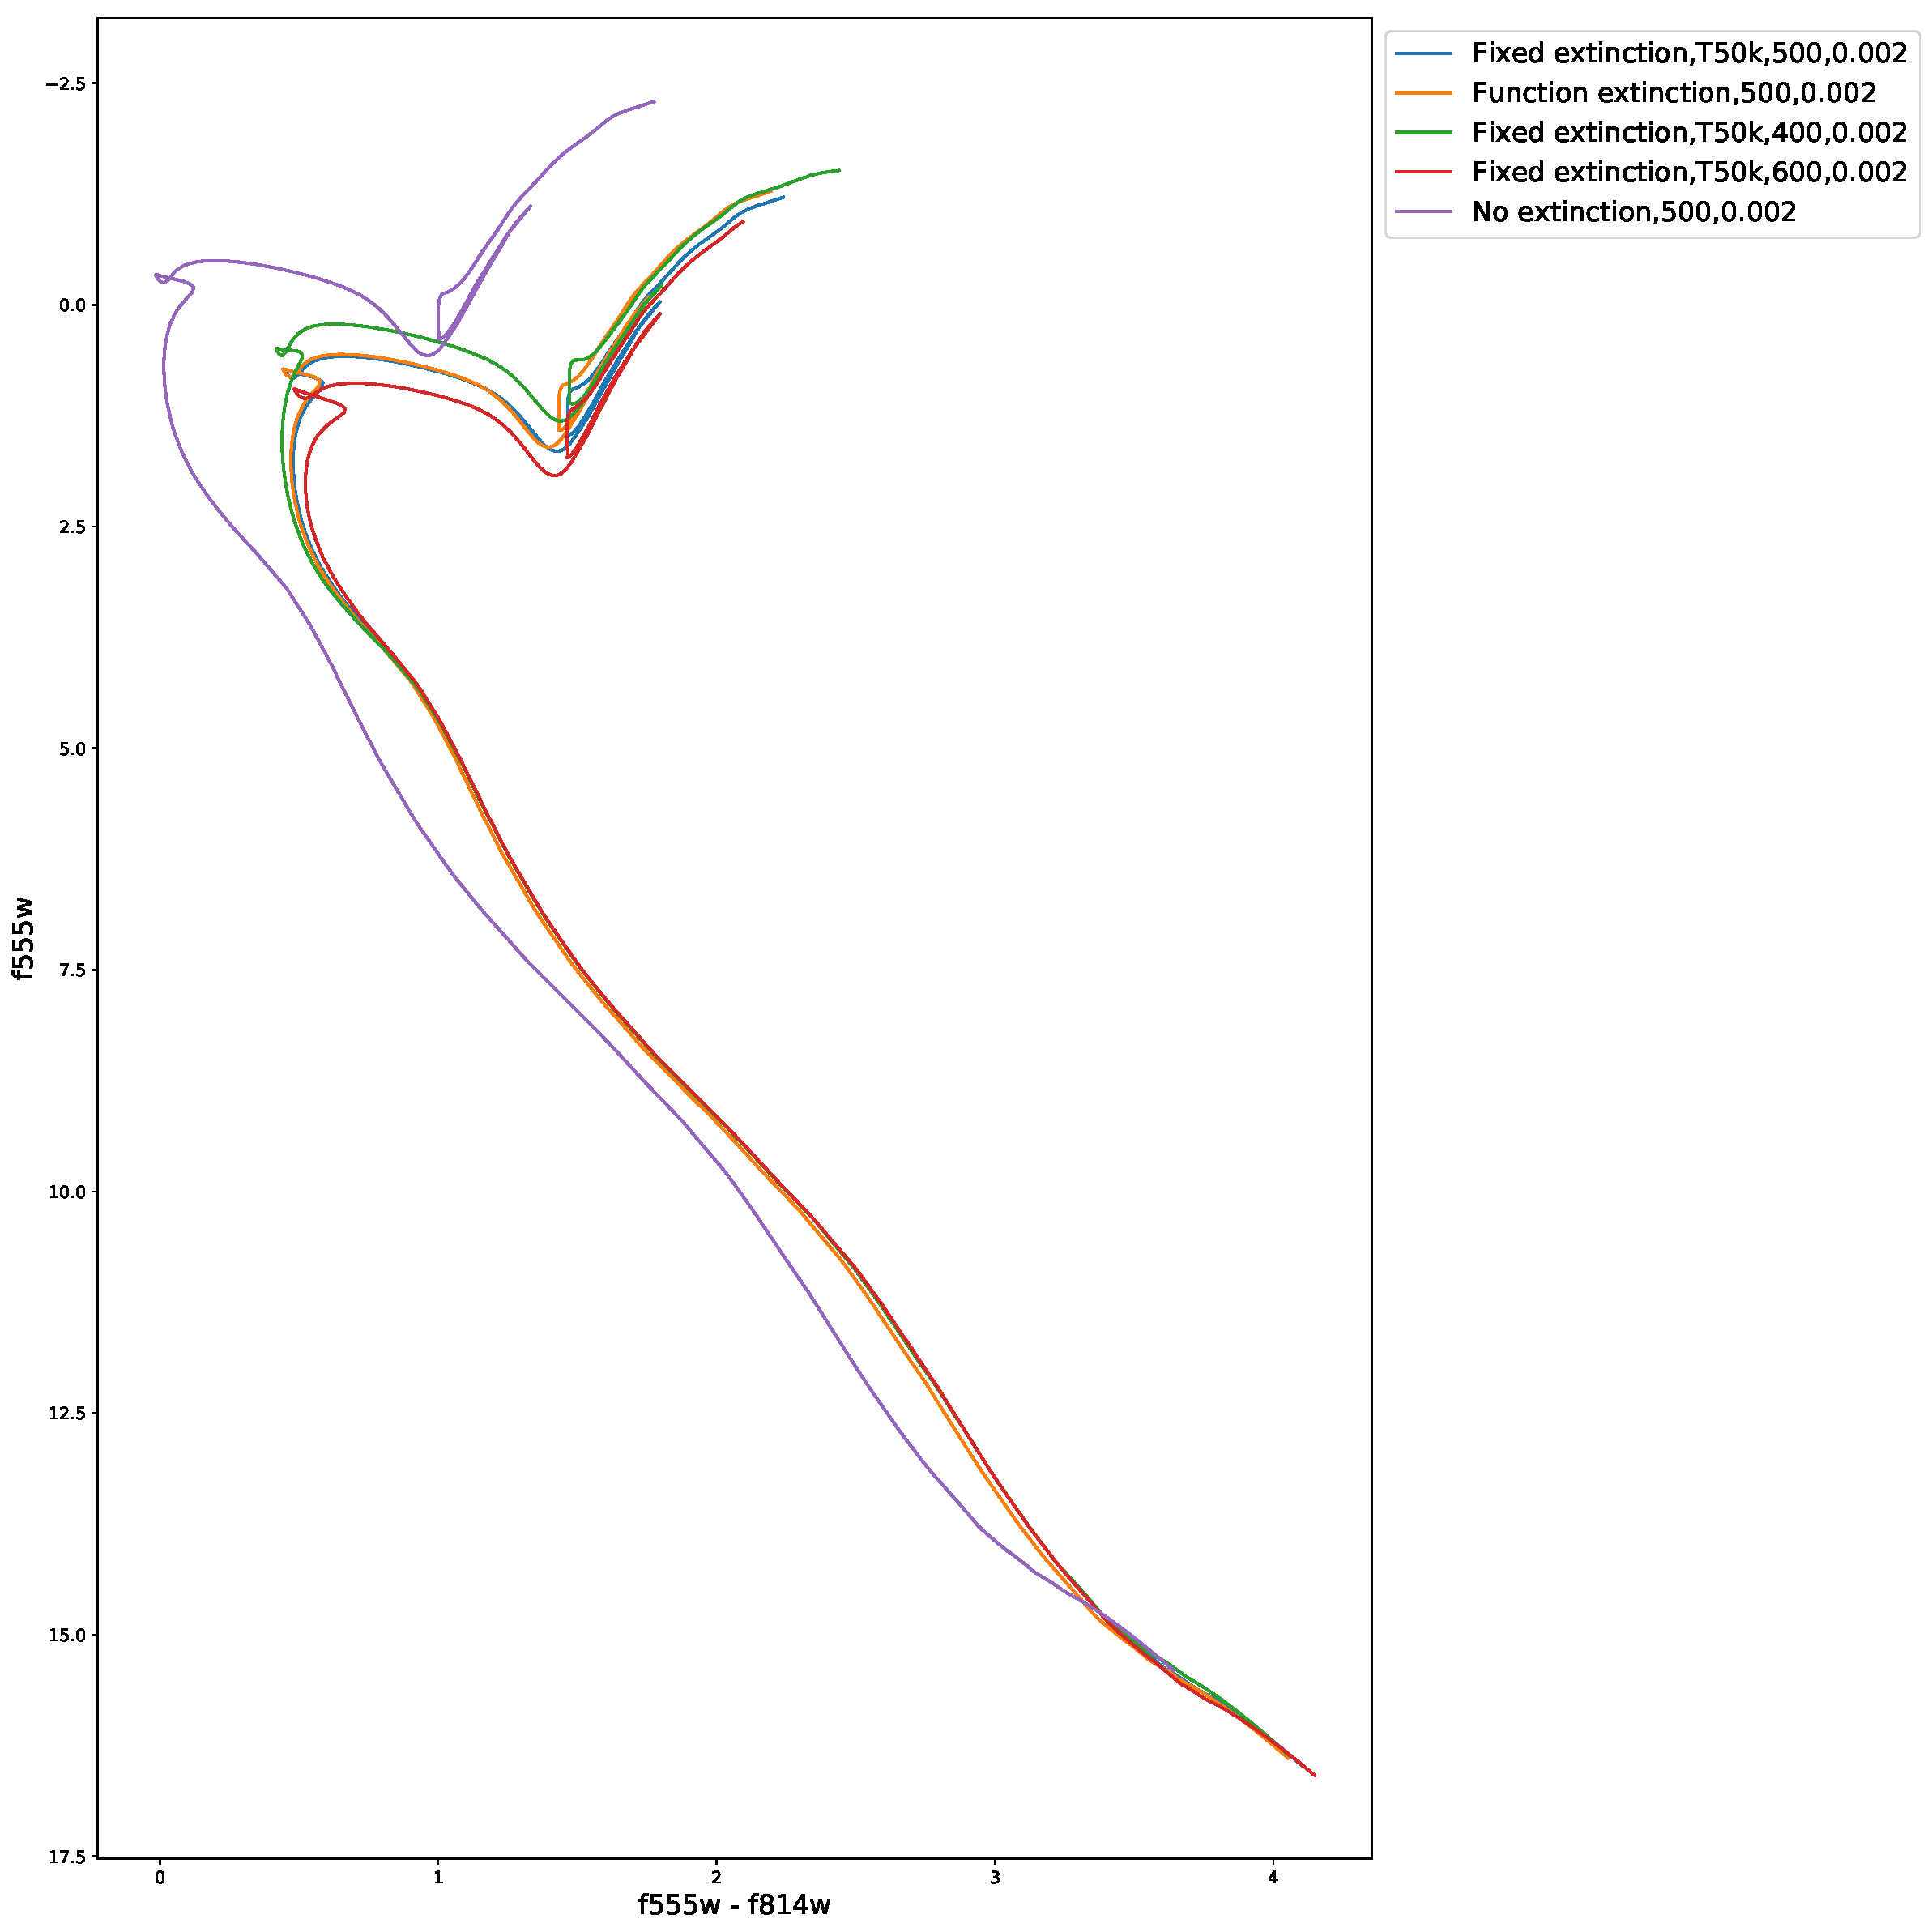
\includegraphics[scale=0.3]{../basti_isochrones_10_13Gyr/Extinction_T50k_FeH0fix_func_f555w_f555wmf814w_500_400_600_Myr_FeH_0p002_ref_noext_Av_1p0.pdf}
\caption{Ratios of $A_{X}/A{V}$ values for different $Z$ values compared with solar metallicity data at log($g$) = 5.0}
\label{wfc3_isoc1_T50k}
\end{center}
\end{figure}

\begin{figure}[h]
\begin{center}
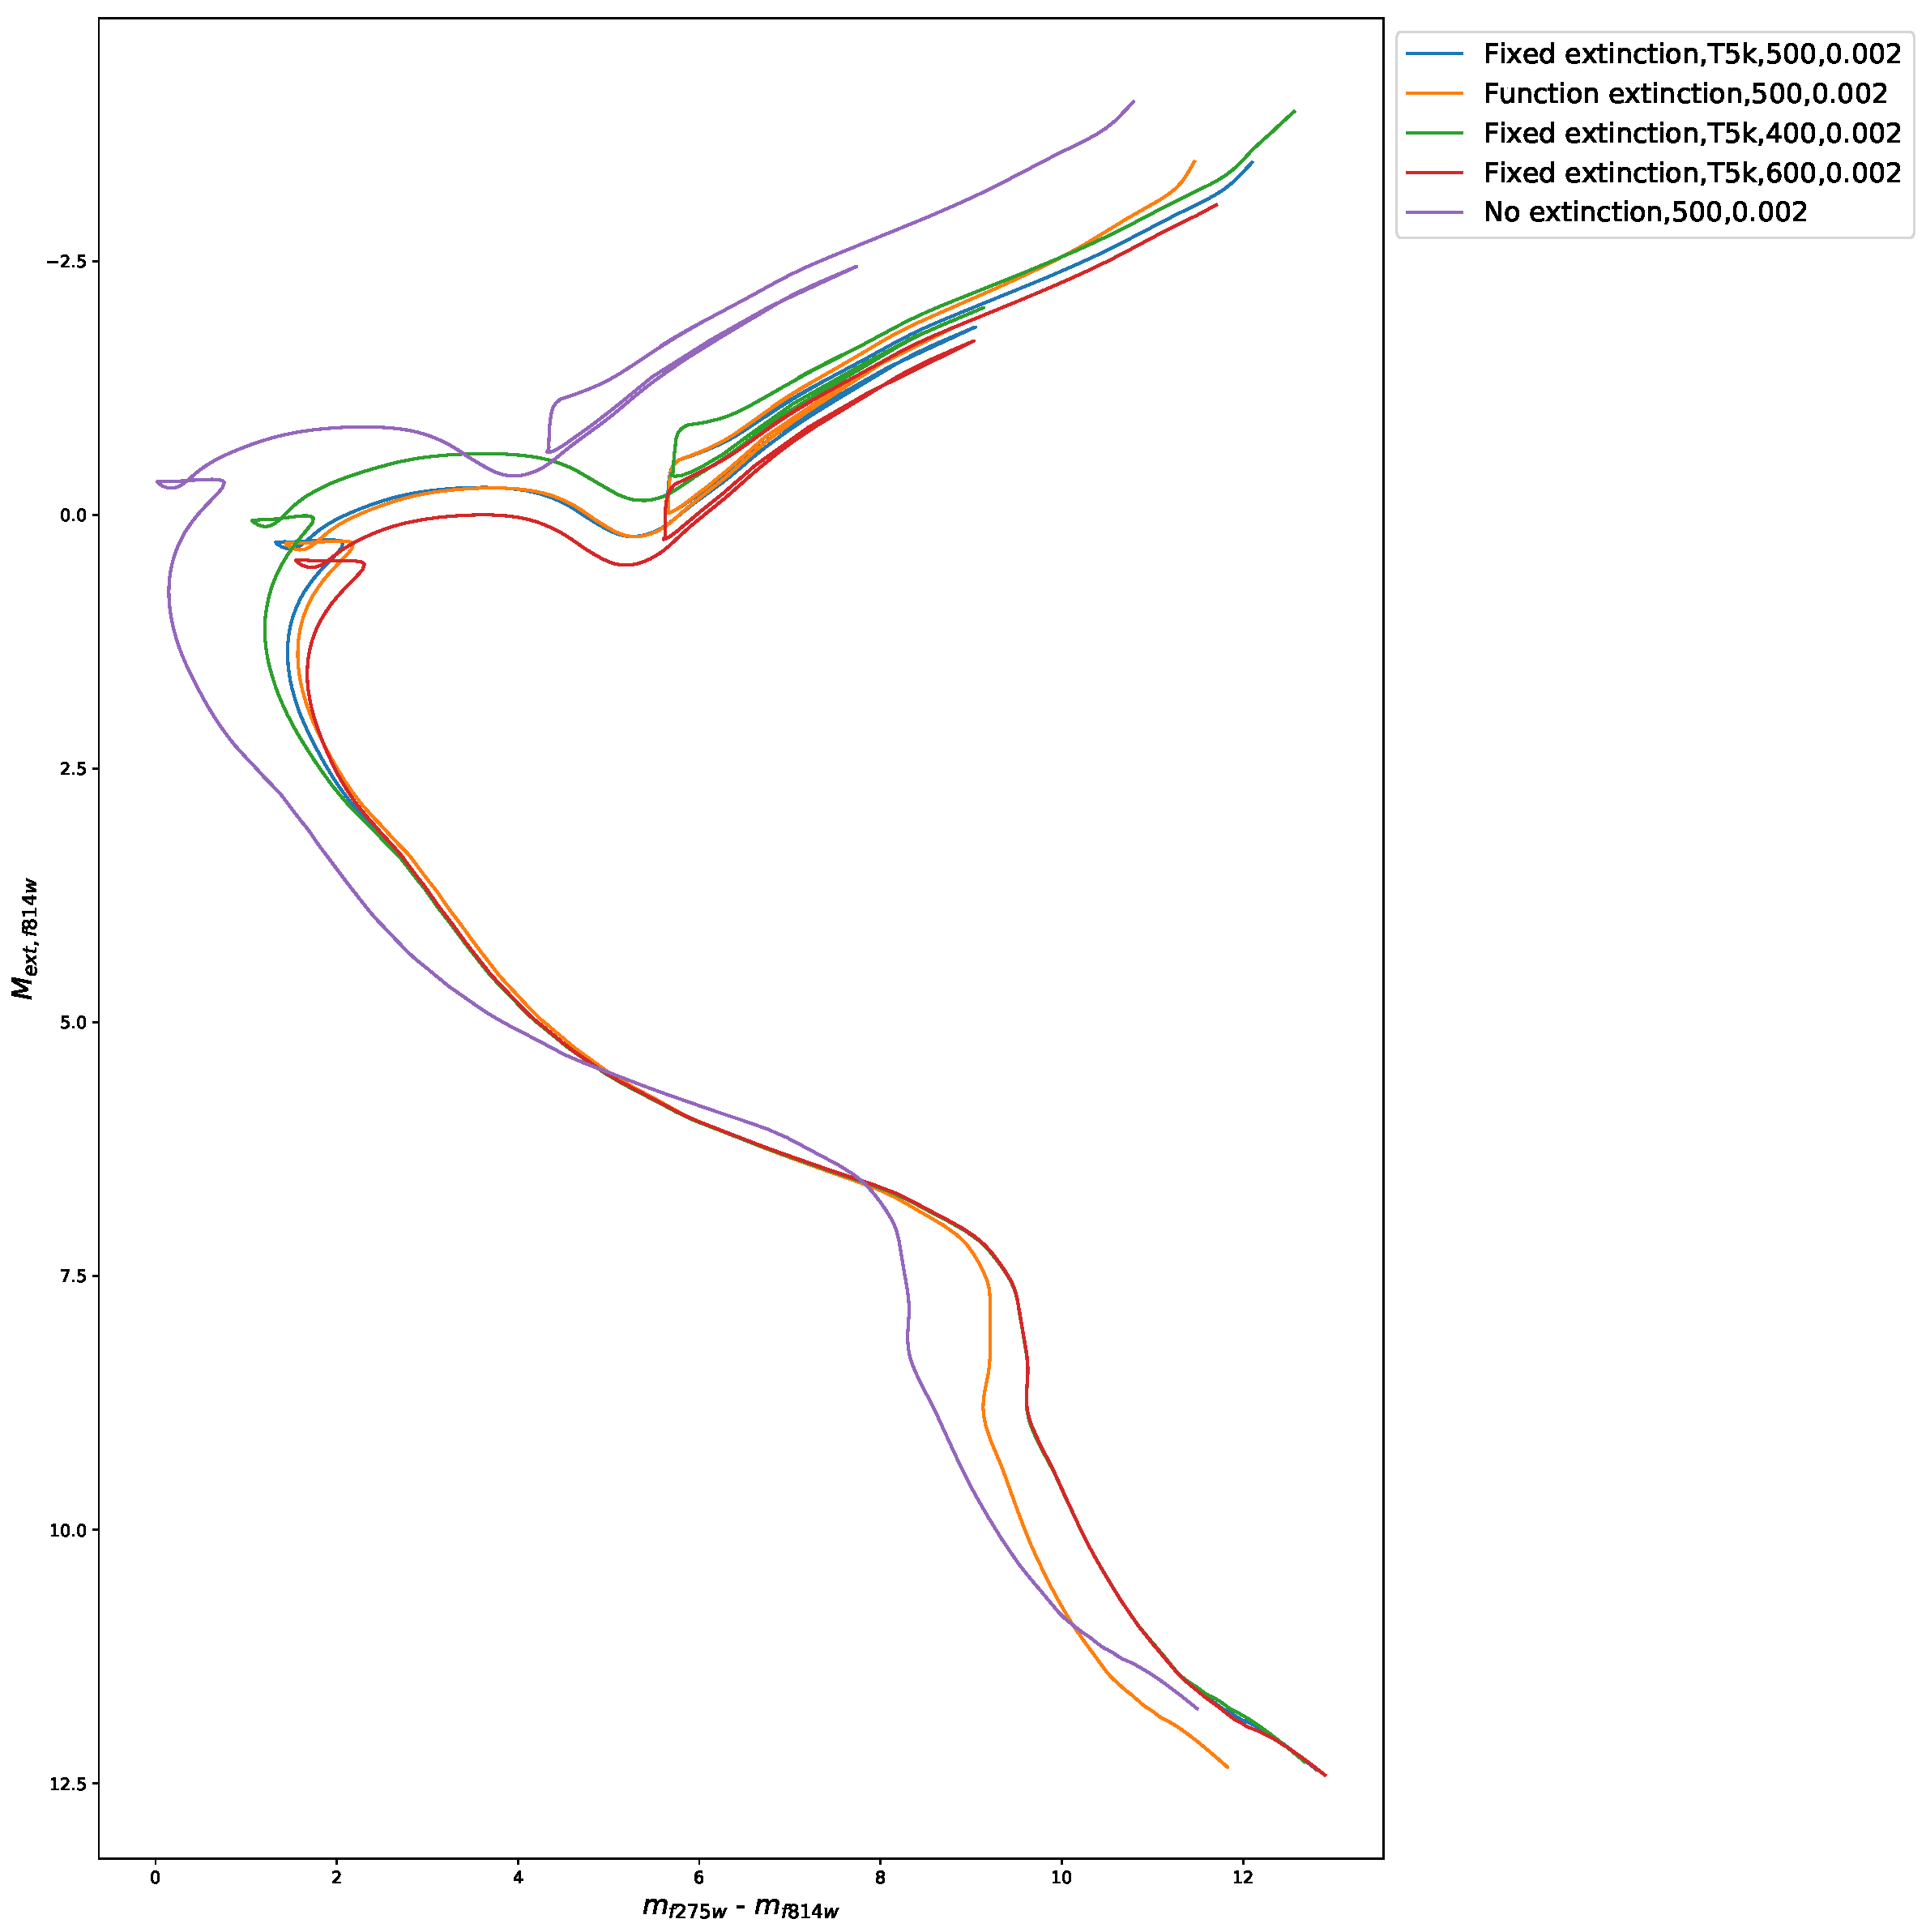
\includegraphics[scale=0.3]{../basti_isochrones_10_13Gyr/Extinction_T5k_FeH0fix_func_f814w_f275wmf814w_500_400_600_Myr_FeH_0p002_ref_noext_Av_1p0.pdf}
\caption{Ratios of $A_{X}/A{V}$ values for different $Z$ values compared with solar metallicity data at log($g$) = 5.0}
\label{wfc3_isoc2_T5k}
\end{center}
\end{figure}

\begin{figure}[h]
\begin{center}
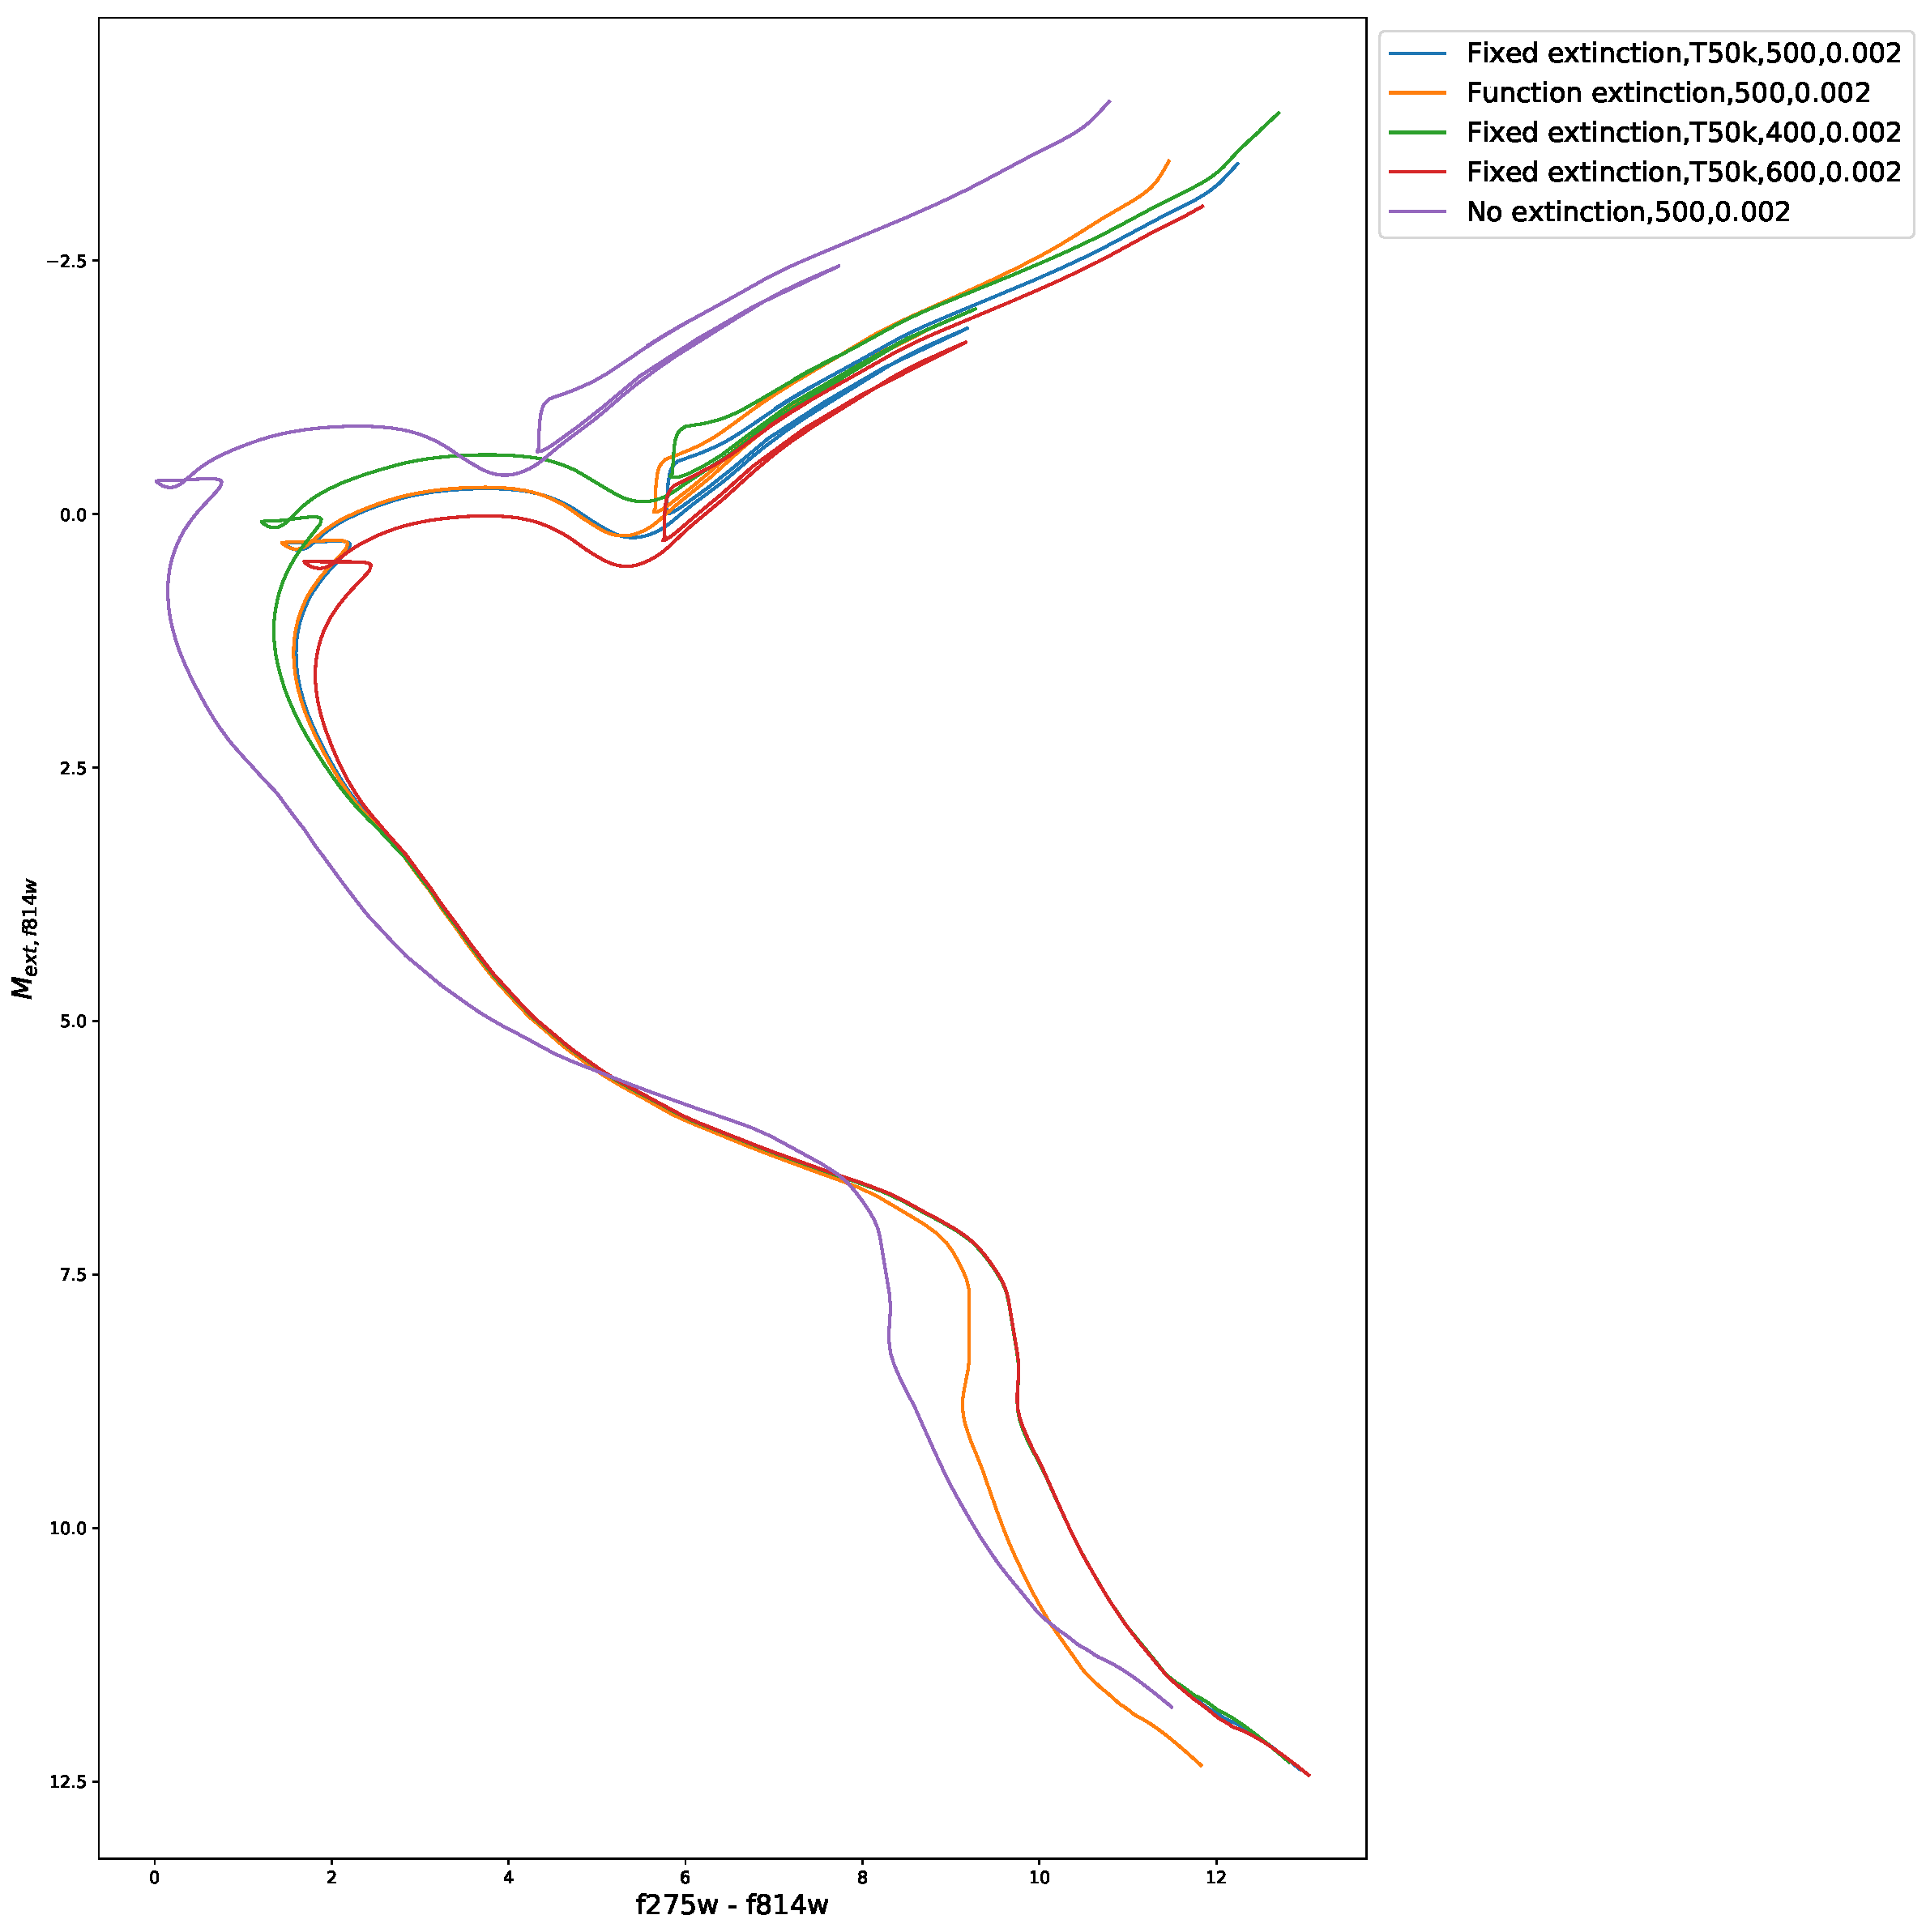
\includegraphics[scale=0.3]{../basti_isochrones_10_13Gyr/Extinction_T50k_FeH0fix_func_f814w_f275wmf814w_500_400_600_Myr_FeH_0p002_ref_noext_Av_1p0.pdf}
\caption{Ratios of $A_{X}/A{V}$ values for different $Z$ values compared with solar metallicity data at log($g$) = 5.0}
\label{wfc3_isoc2_T50k}
\end{center}
\end{figure}

\subsubsection{Gaia} \label{Gaia_isoc}

\begin{figure}[h]
\begin{center}
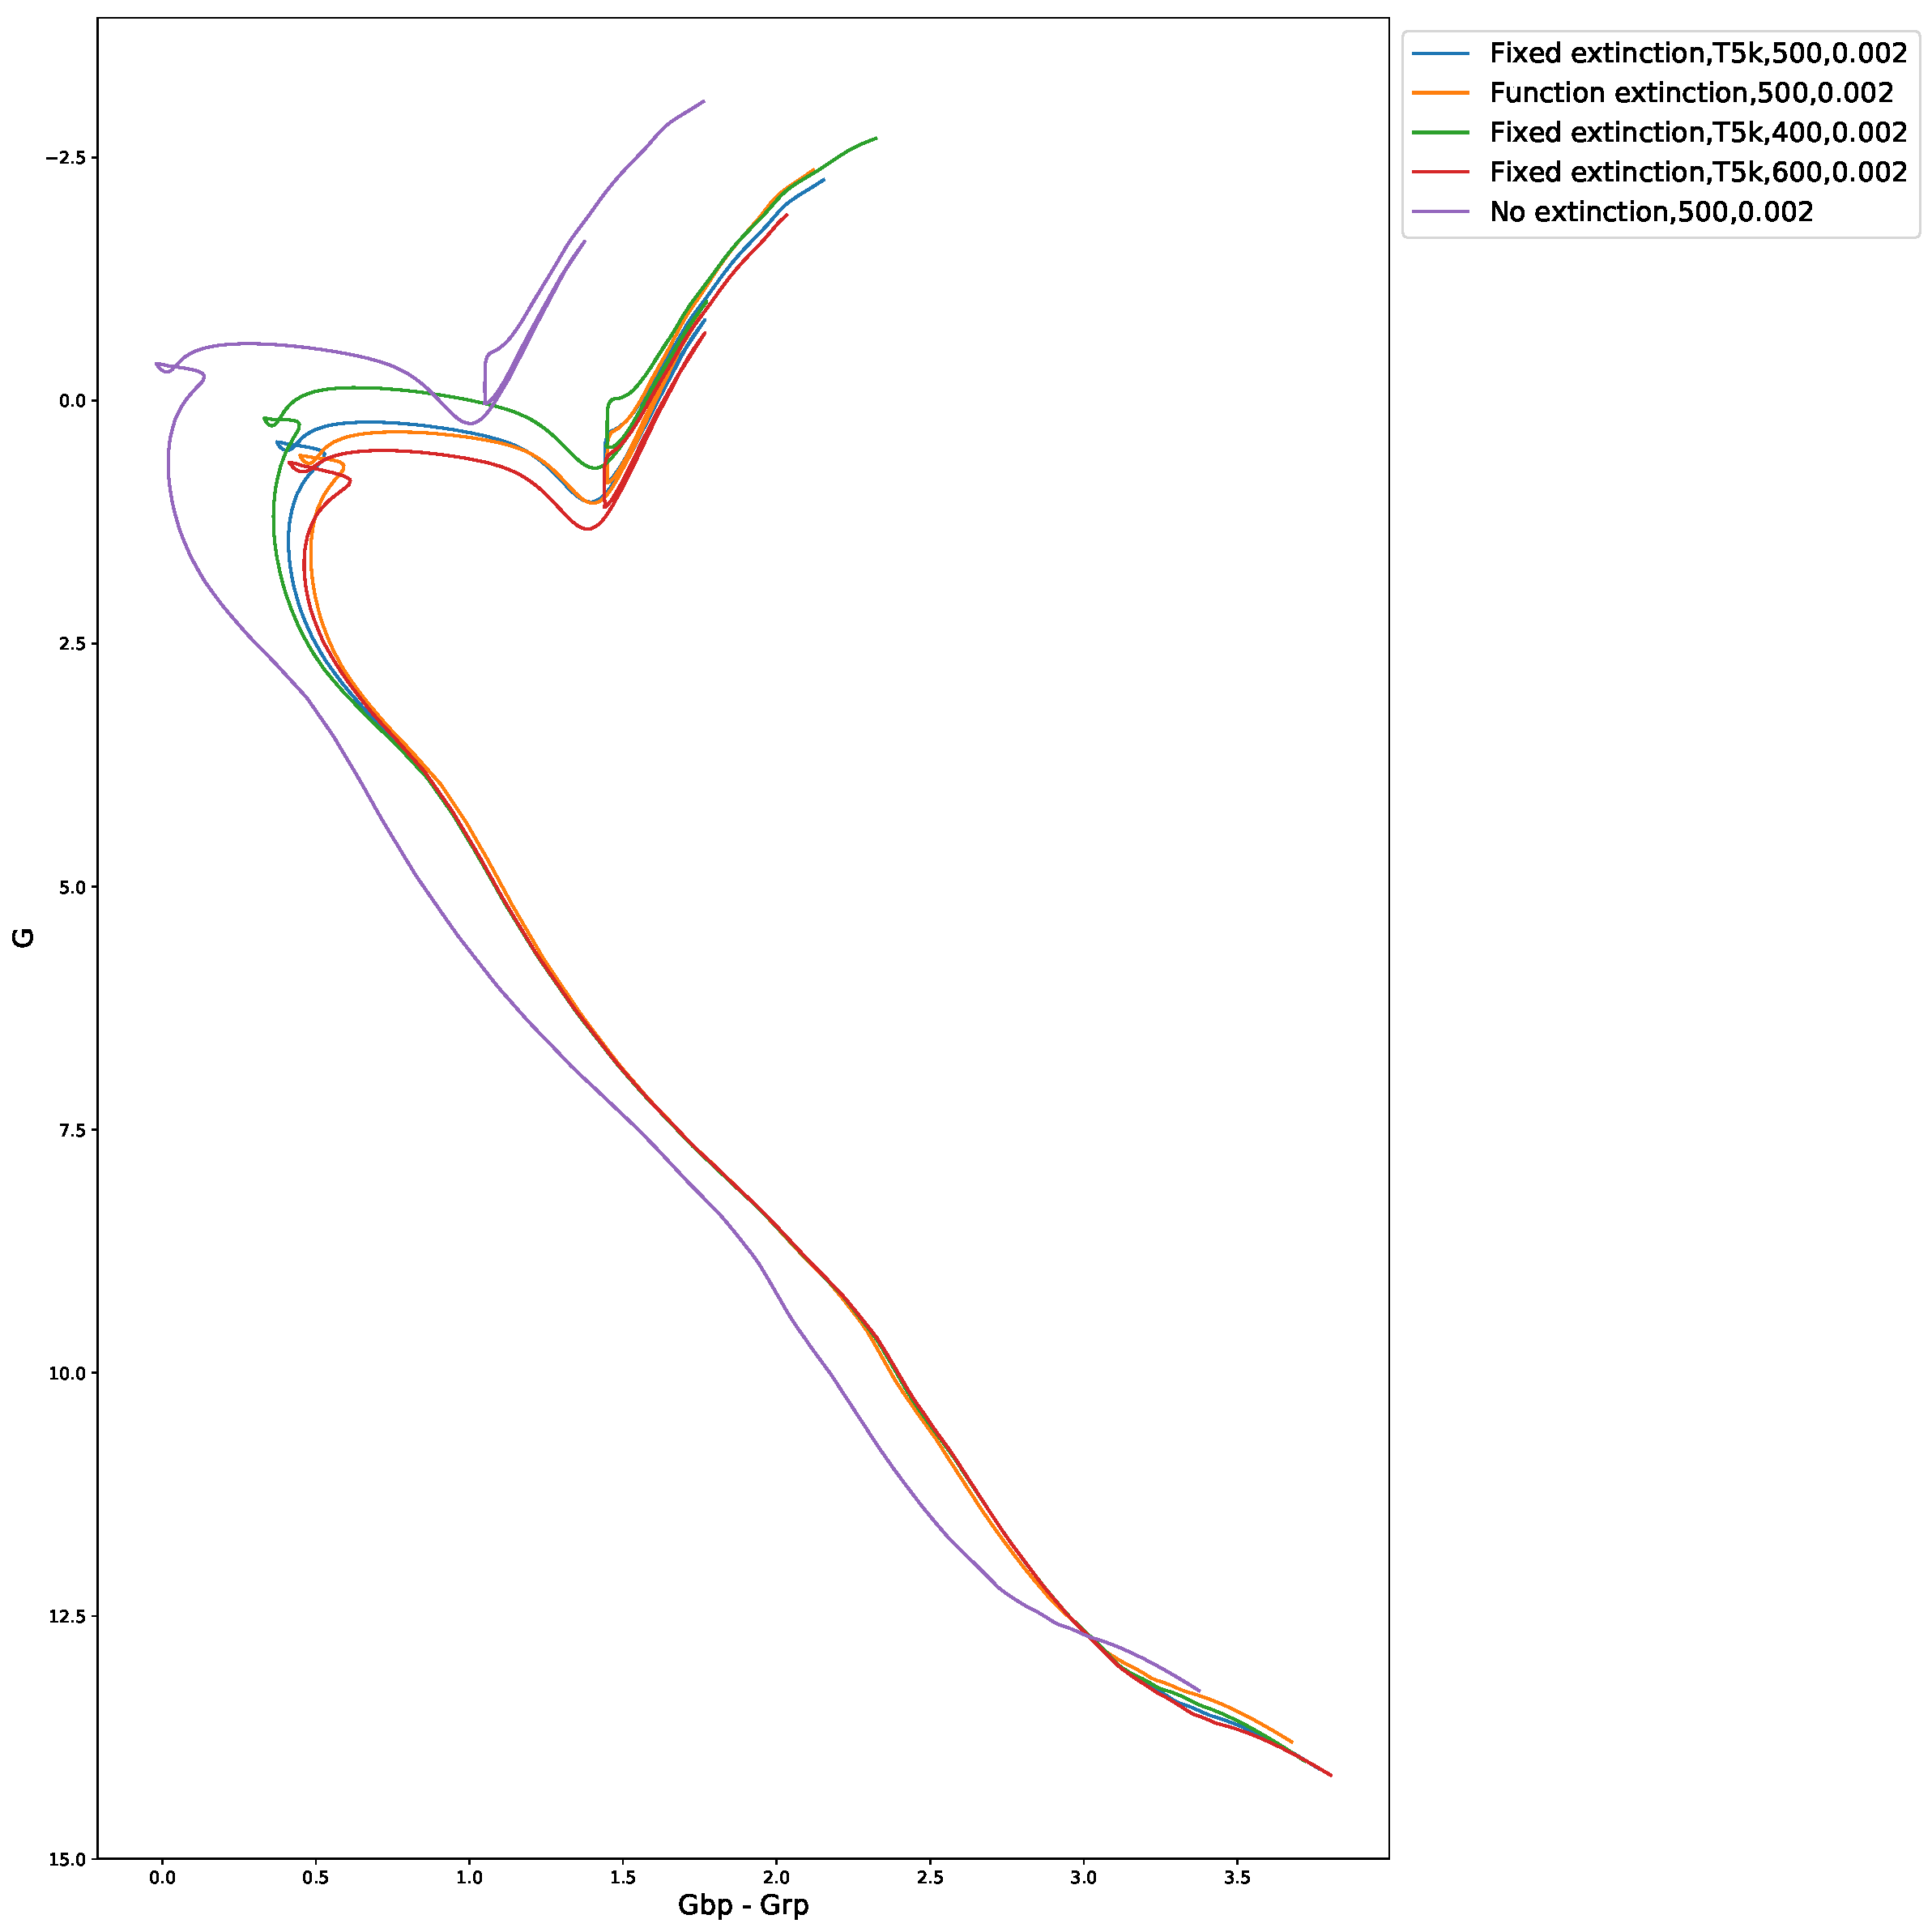
\includegraphics[scale=0.3]{../basti_isochrones_10_13Gyr/Extinction_T5k_FeH0fix_func_G_GbpmGrp_500_400_600_Myr_FeH_0p002_ref_noext_Av_1p0.pdf}
\caption{Ratios of $A_{X}/A{V}$ values for different $Z$ values compared with solar metallicity data at log($g$) = 5.0}
\label{gaia_isoc_T5k}
\end{center}
\end{figure}

\begin{figure}[h]
\begin{center}
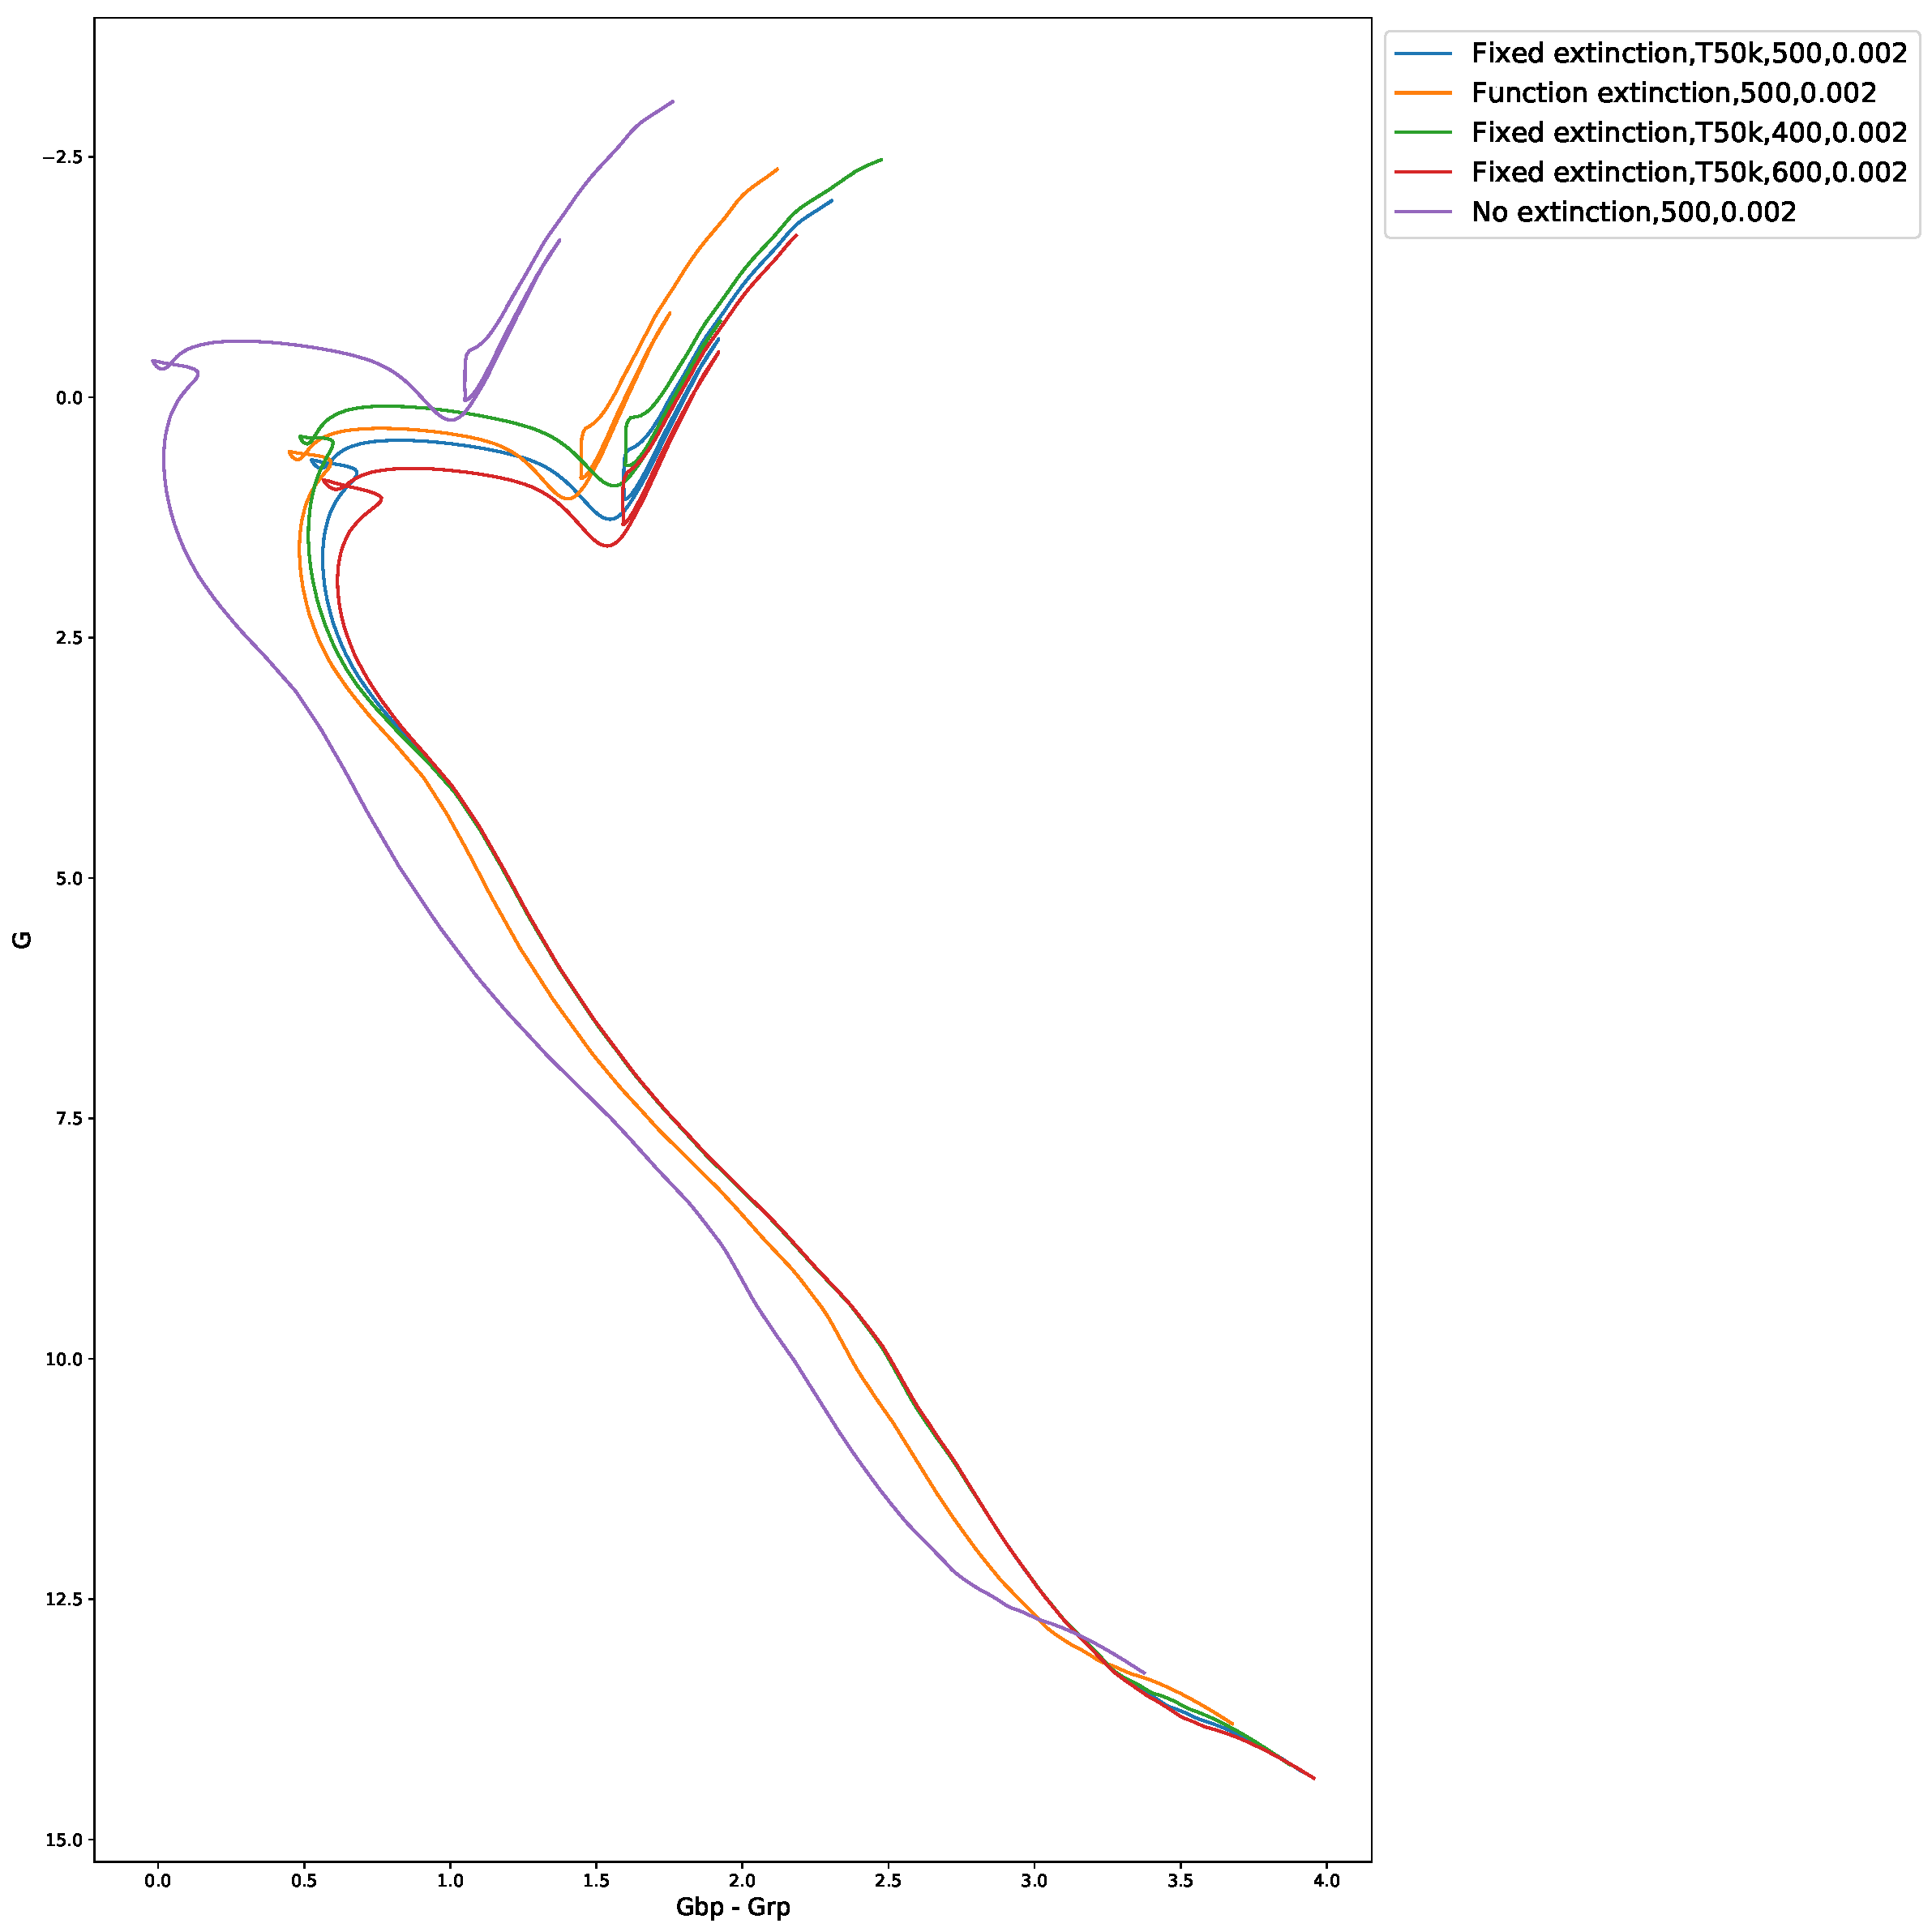
\includegraphics[scale=0.3]{../basti_isochrones_10_13Gyr/Extinction_T50k_FeH0fix_func_G_GbpmGrp_500_400_600_Myr_FeH_0p002_ref_noext_Av_1p0.pdf}
\caption{Ratios of $A_{X}/A{V}$ values for different $Z$ values compared with solar metallicity data at log($g$) = 5.0}
\label{gaia_isoc_T50k}
\end{center}
\end{figure}

\subsection{Test case: NGC 6793}
To test the effects of the difference in treatment of $A_{X}/A{V}$, both cases were employed to predict the isochrone ***parameters of the open cluster NGC 6793.

\subsubsection{Observational background}
NGC 6793 has little information available compared to many other open clusters. Two estimates for observational properties of the cluster have been published and are listed in Table \ref{NGC6793_obs}.

\begin{table}
\begin{center}
\begin{tabular}{ccc}
\hline
%\multirow{2}{*}{System} & \multirow{2}{*}{Filter} & \multirow{2}{*}{$A_{1}$ function} & \multicolumn{3}{c}{$A_{1}$ coefficients} \\ \cline{4-6}
%\textbf{Filter} \\
Cluster property & K05 & B18
\hline
Distance modulus / mag & 10.73 & 8.894 \\
-> distance / pc & 1400 & 601 \\
log(age / yr) & 8.64 & 8.78 \\
-> Age / Myr & 437 & 603 \\
$E(B-V)$ / mag & 0.17 & 0.272 \\
[Fe/H] & ? & ? \\
Members & ? & 465 (271 with Gaia photometry) \\
\hline

\end{tabular}
\caption{Observational parameters for NGC 6793, according to \cite{2005A&A...438.1163K} (WEBDA archive page) and \cite{2018A&A...616A..10G}}
\label{NGC6793_obs}
\end{center}
\end{table}

\subsubsection{Comparison of extinction methods}
The Gaia DR2 dataset, containing the parallaxes and apparent magnitudes (in all three Gaia filters) for 338 objects tagged as belonging to NGC 6793, was obtained. The number of objects is greater than the 271 photometric Gaia objects found by \cite{2018A&A...616A..10G}. There were significant variations in the observed parallaxes of individual stars, far beyond the maximum cluster radii expected (\cite{2006A&A...456..523S} - general open cluster properties).

There are highly significant errors for the individual objects in the Gaia data propagation, even when assuming the only source of error is from  parallax measurements (see Figure \ref{ngc_errorbars}). The magnitude of the errorbars dwarf any changes in isochrones due to extinction coefficient treatments.

All, as shown in Section****, the isochrones are sensitive both to the reference extinction coefficient value $A_{V}$ and to the value of $A_{X}/A_{V}$ for the fixed case. Some individual parts of the isochrones relevant to this study are additionally sensitive to other isochrone parameters:

\begin{enumerate}
%, but metallicity has a smaller effect
\item The position of the MSTO is sensitive to the treatment of $A_{X}/A_{V}$, as shown in Section****, and the isochrone age.
\item The position of the lower main sequence is significantly more sensitive to metallicity than other parts of the isochrone.
\end{enumerate}

\begin{figure}[h]
\begin{center}
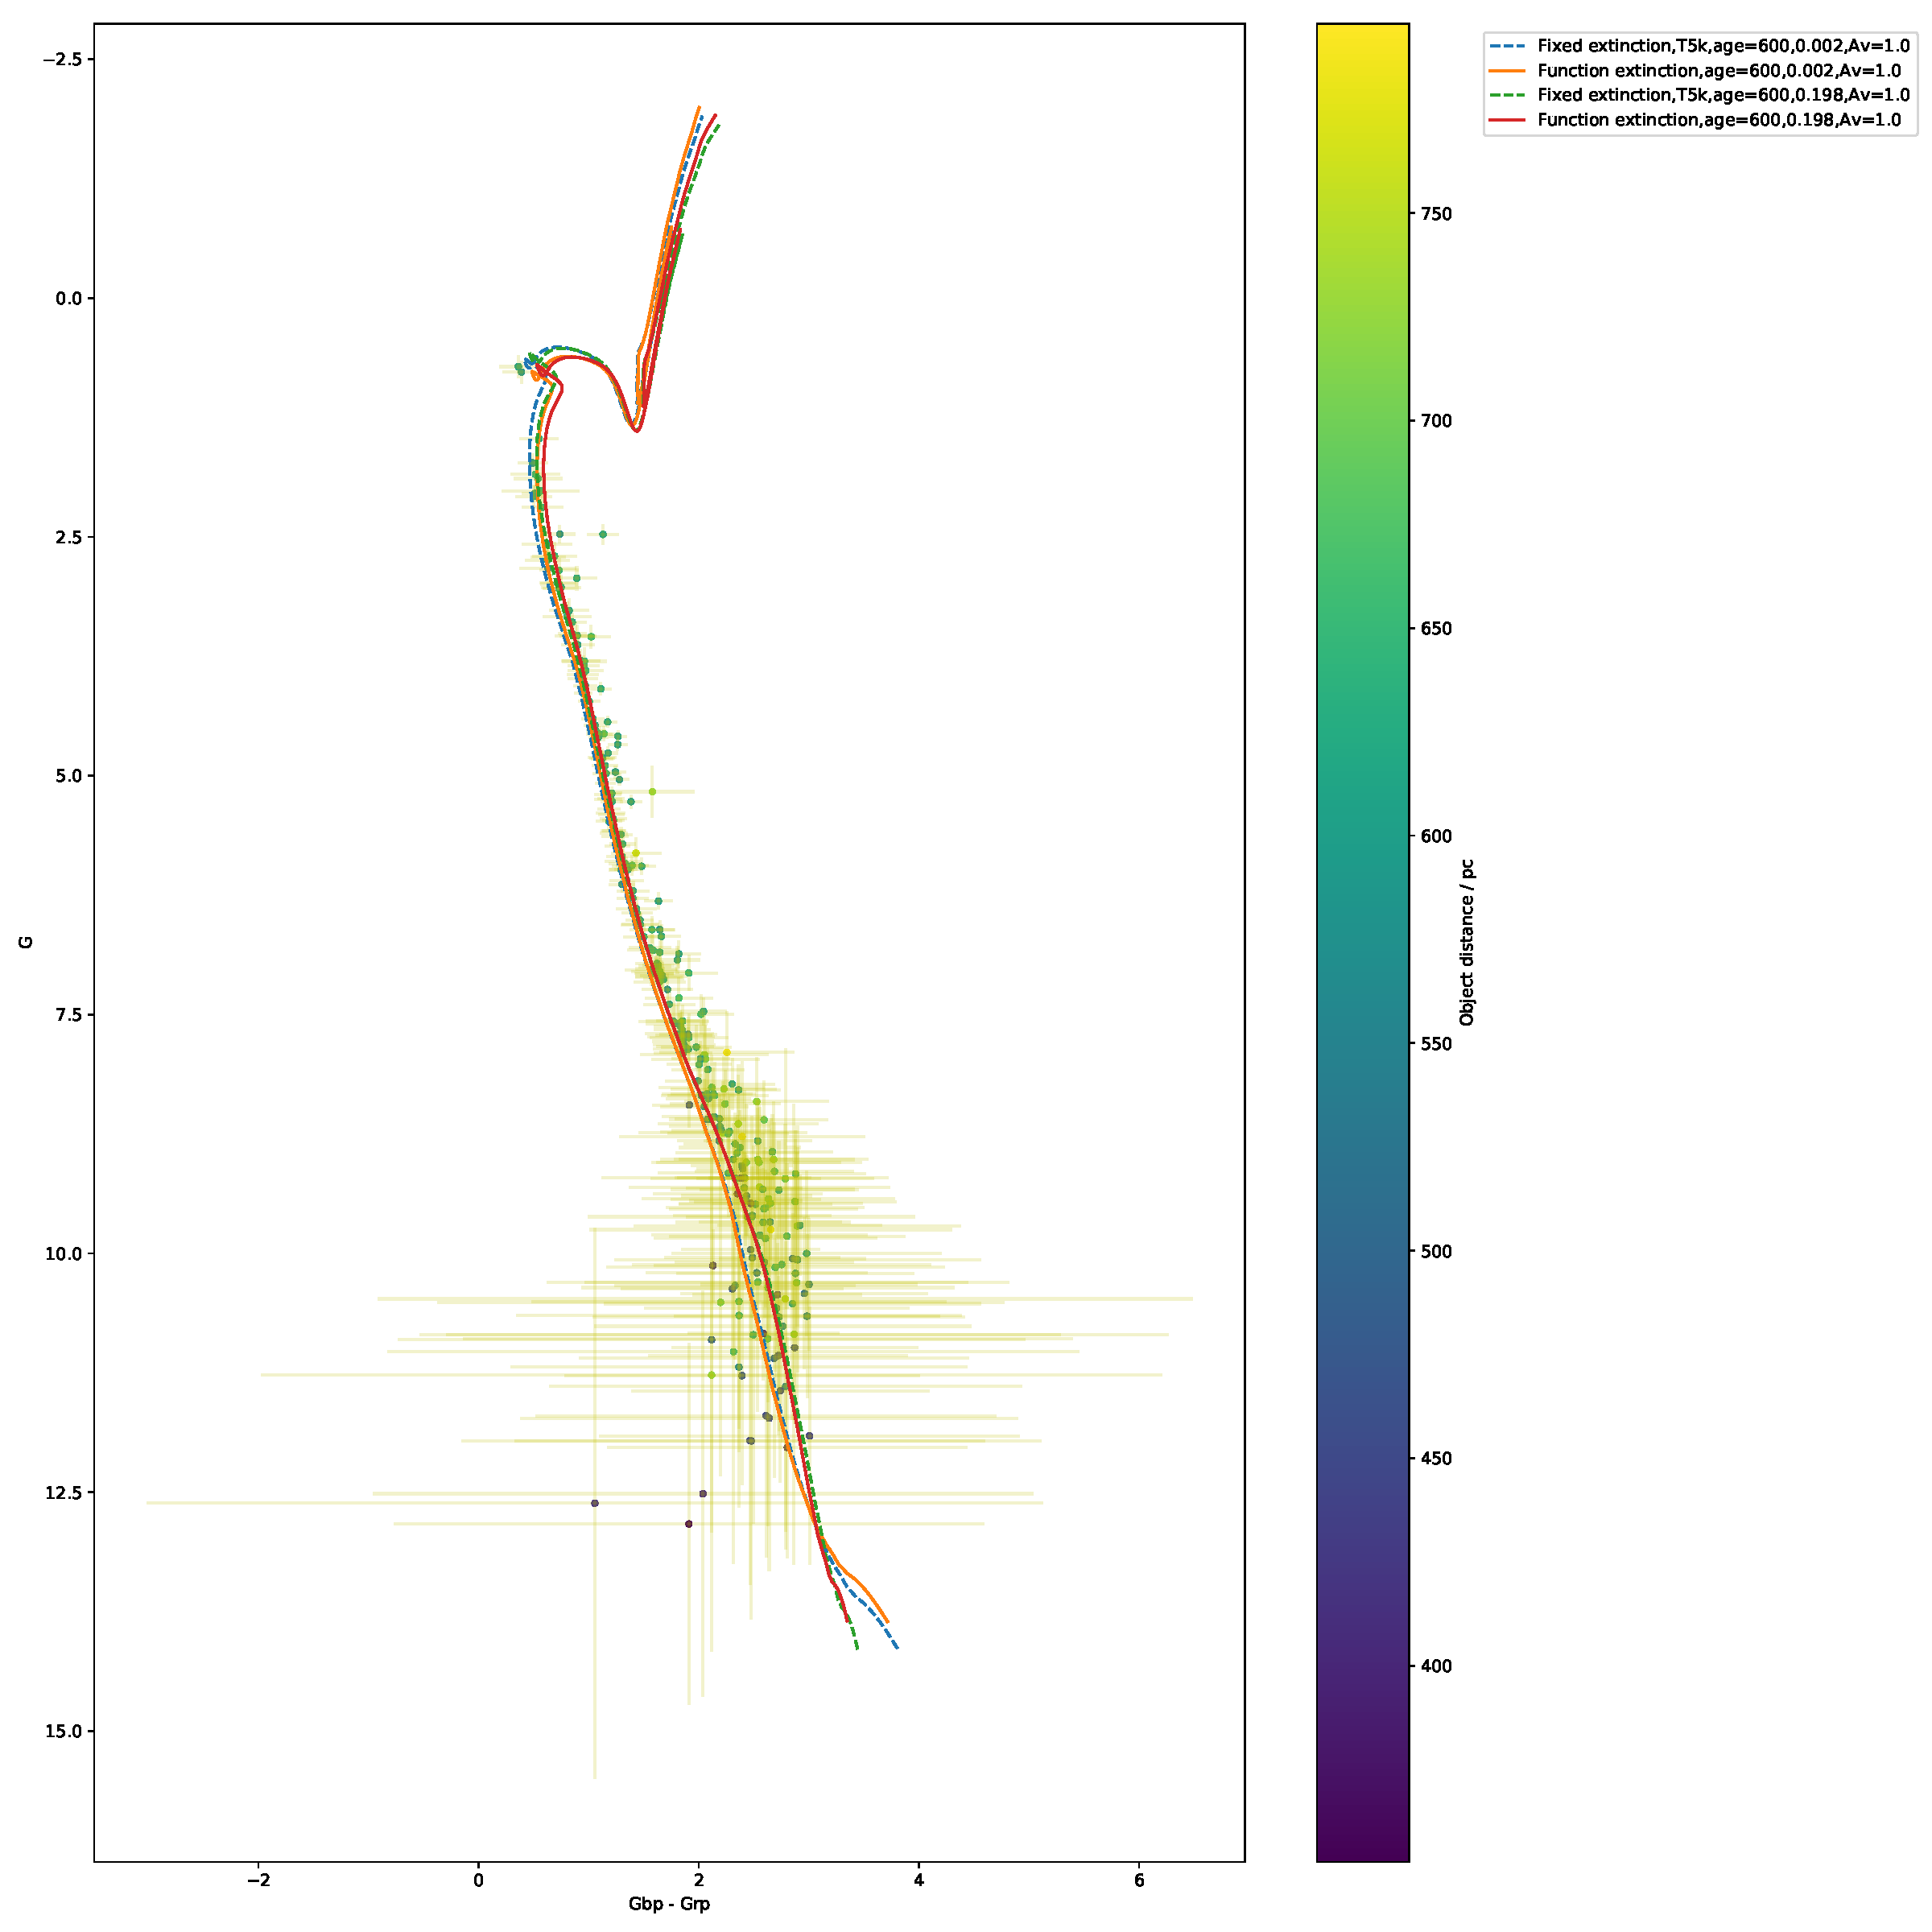
\includegraphics[scale=0.3]{../NGC_6793_CMD_FeH_0p002_0p198_Av_1p0_600Myr_isochrones_both_errorbars_T5k.pdf}
\caption{Gaia CMD of NGC 6793 with errorbars included.}
\label{ngc_errorbars}
\end{center}
\end{figure}

\section{Conclusion}
\subsection{Future work}
\bibliographystyle{mnras} % unsrtnat
\bibliography{mphil_thesis}

\end{document}